
\documentclass[compress]{beamer}

%\usepackage{beamerthemesplit}
\usepackage{xmpmulti}

\usepackage{graphicx,float,wrapfig, bbm}
\usepackage{amsfonts, bbold, comment}
\usepackage{mdwlist}
\usepackage{subfigure}
\usepackage{colortbl}

\usepackage{multirow}

\pgfdeclareimage[width=\paperwidth]{mybackground}{../../common/boulder.pdf}

\newcommand{\e}[2]{\mathbb{E}_{#1}\left[ #2 \right] }
\newcommand{\ind}[1]{\mathbb{I}\left[ #1 \right] }
\newcommand{\ex}[1]{\mbox{exp}\left\{ #1\right\} }
%\newcommand{\g}{\, | \,}
\newcommand{\citename}[1]{#1 }

\newcommand{\greentext}[1]{\textcolor{caribbeangreen}{#1}}
\newcommand{\yellowtext}[1]{\textcolor{amber}{#1}}
\newcommand{\redtext}[1]{\textcolor{red}{#1}}
\newcommand{\bluetext}[1]{\textcolor{blue}{#1}}

\newcommand{\bm}[1]{\mbox{\boldmath$#1$}}
\newcommand{\Dir}{\mathrm{Dir}}
\newcommand{\Mult}{\mathrm{Mult}}
\newcommand{\g}[1]{\Gamma \left( #1 \right)}
\newcommand{\paragraph}[1]{ \vskip 1cm {\bf \large #1}}

\newcommand{\tb}[1]{\textbf{#1}}
\newcommand{\subtwo}[2]{_{#1, #2}}
\newcommand{\subthree}[3]{_{#1, #2, #3}}
\newcommand{\minussubtwo}[2]{_{-{#1, #2}}}
\newcommand{\minussubthree}[3]{_{-{#1, #2, #3}}}
\newcommand{\suptwo}[2]{^{#1, #2}}
\newcommand{\supthree}[3]{^{#1, #2, #3}}
\newcommand{\minussuptwo}[2]{^{-{#1, #2}}}
\newcommand{\minussupthree}[3]{^{-{#1, #2, #3}}}
\newcommand{\prior}[1]{\mathcal{B}#1} % to be revised

\newcommand{\gfx}[2]{
\begin{center}
	\includegraphics[width=#2\linewidth]{teaparty/figures/#1}
\end{center}
}


\usetheme[bullet=circle,                     % Use circles instead of squares for bullets.
          titleline=true,                    % Show a line below the frame title.
          showdate=true,                     % show the date on the title page
          alternativetitlepage=true,         % Use the fancy title page.
          titlepagelogo=general_figures/culogo,              % Logo for the first page.
          % Logo for the header on first page.
          headerlogo=general_figures/boulder_cs,
          ]{UCBoulder}

\usecolortheme{ucdblack}
\title[Tea Party in the House]{Tea Party in the House: A Hierarchical Ideal Point Topic Model
  and Its Application to Republican Legislators in the 112\textsuperscript{th} Congress}
\author[Nguyen, Miler, Boyd-Graber, Resnik]{Viet-An Nguyen, Kristina Miler, Jordan Boyd-Graber, and Philip Resnik}
\date{August 2015}

\institute[Boulder] % (optional, but mostly needed)
{University of Colorado Boulder}

\AtBeginSection[] % "Beamer, do the following at the start of every section"
{ \begin{frame} \frametitle{Outline} % make a frame titled "Outline"
\tableofcontents[currentsection] % show TOC and highlight current section
\end{frame} }

\begin{document}

\frame{
\titlepage
\tiny
}

\begin{frame}{}

  \begin{columns}
    \column{.5\linewidth}
      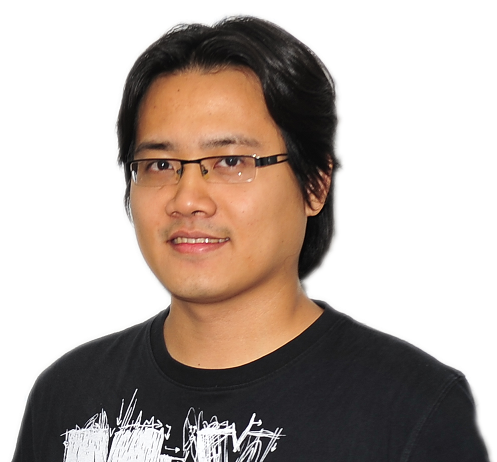
\includegraphics[width=.9\linewidth]{general_figures/an}
    \column{.5\linewidth}
      \begin{itemize}
        \item Former PhD student at Maryland
        \item Now at Facebook
        \item Visa issues
      \end{itemize}
  \end{columns}

\end{frame}

\section[Multi-dimensional Ideal Points from Roll-call Votes and Text]{Multi-dimensional Ideal Points from Roll-call Votes and Text}%


\section{Motivation}

\begin{frame}{Representing Elected Officials: Ideal Points}
  \gfx{dw_nominate}{.7}
  \pause
  An essential tool in political science: distinguish trends and characterize subgroups
\end{frame}


\frame{
\frametitle{Evaluation: Tea Party in the House}
    \begin{block}{The Tea Party}
    \small
    \begin{itemize*}
      \item Recent American political movement supporting more freedom, smaller government, lower tax
      \item Played an important role in recent electoral politics, especially within the Republican
      Party
      \item Organizations:
      \begin{itemize}
        \item Institutional: Tea Party Caucus
        \item Other: Tea Party Express, Tea Party Patriots, Freedom Works
      \end{itemize}
      \item ``\textbf{Conventional views of ideology as a single--dimensional, left�-right
          spectrum experience great difficulty in understanding or explaining the Tea Party.}''

        \hfill \cite[ARPS]{CarminesARPS15}
    \end{itemize*}
    \end{block}

    \pause
    \vspace{-.2cm}
    \begin{block}{Goal}
    \small
    \begin{itemize*}
      \item Explain Tea Partiers in terms of issues and votes
      \item Identify Tea Partiers from their rhetoric
    \end{itemize*}
    \end{block}
}


\begin{frame}{Not everyone has a voting record}

  \begin{columns}
    \column{.5\linewidth}
    \begin{itemize}
      \item Ideal points estimated based on voting record
      \item Not all candidates have a voting record
        \begin{itemize}
          \item Governors
          \item Entertainers
          \item CEOs
        \end{itemize}
        \pause
       \item But all politicians---by definition---talk
      \end{itemize}
      \column{.25\linewidth}
        \gfx{carson}{.75}
        \gfx{fiorina}{.75}
      \column{.25\linewidth}
        \gfx{walker}{.75}
        \gfx{schwarzenegger}{.75}
  \end{columns}

\end{frame}

\begin{frame}{Let's use whatever data we have}

\begin{columns}
  \column{.6\linewidth}
  \gfx{carson_twitter}{.95}
  \column{.4\linewidth}
  A single model that uses:
  \begin{itemize}
    \item Bill text
    \item Votes
    \item Commentary
  \end{itemize}
  to map political actors to the same continuous space.
\end{columns}
\end{frame}

\section{Ideal Point Review}

\frame{
    \frametitle{One-dimensional Ideal Point using Votes}
    \begin{figure}
      \centering
        \only<1>{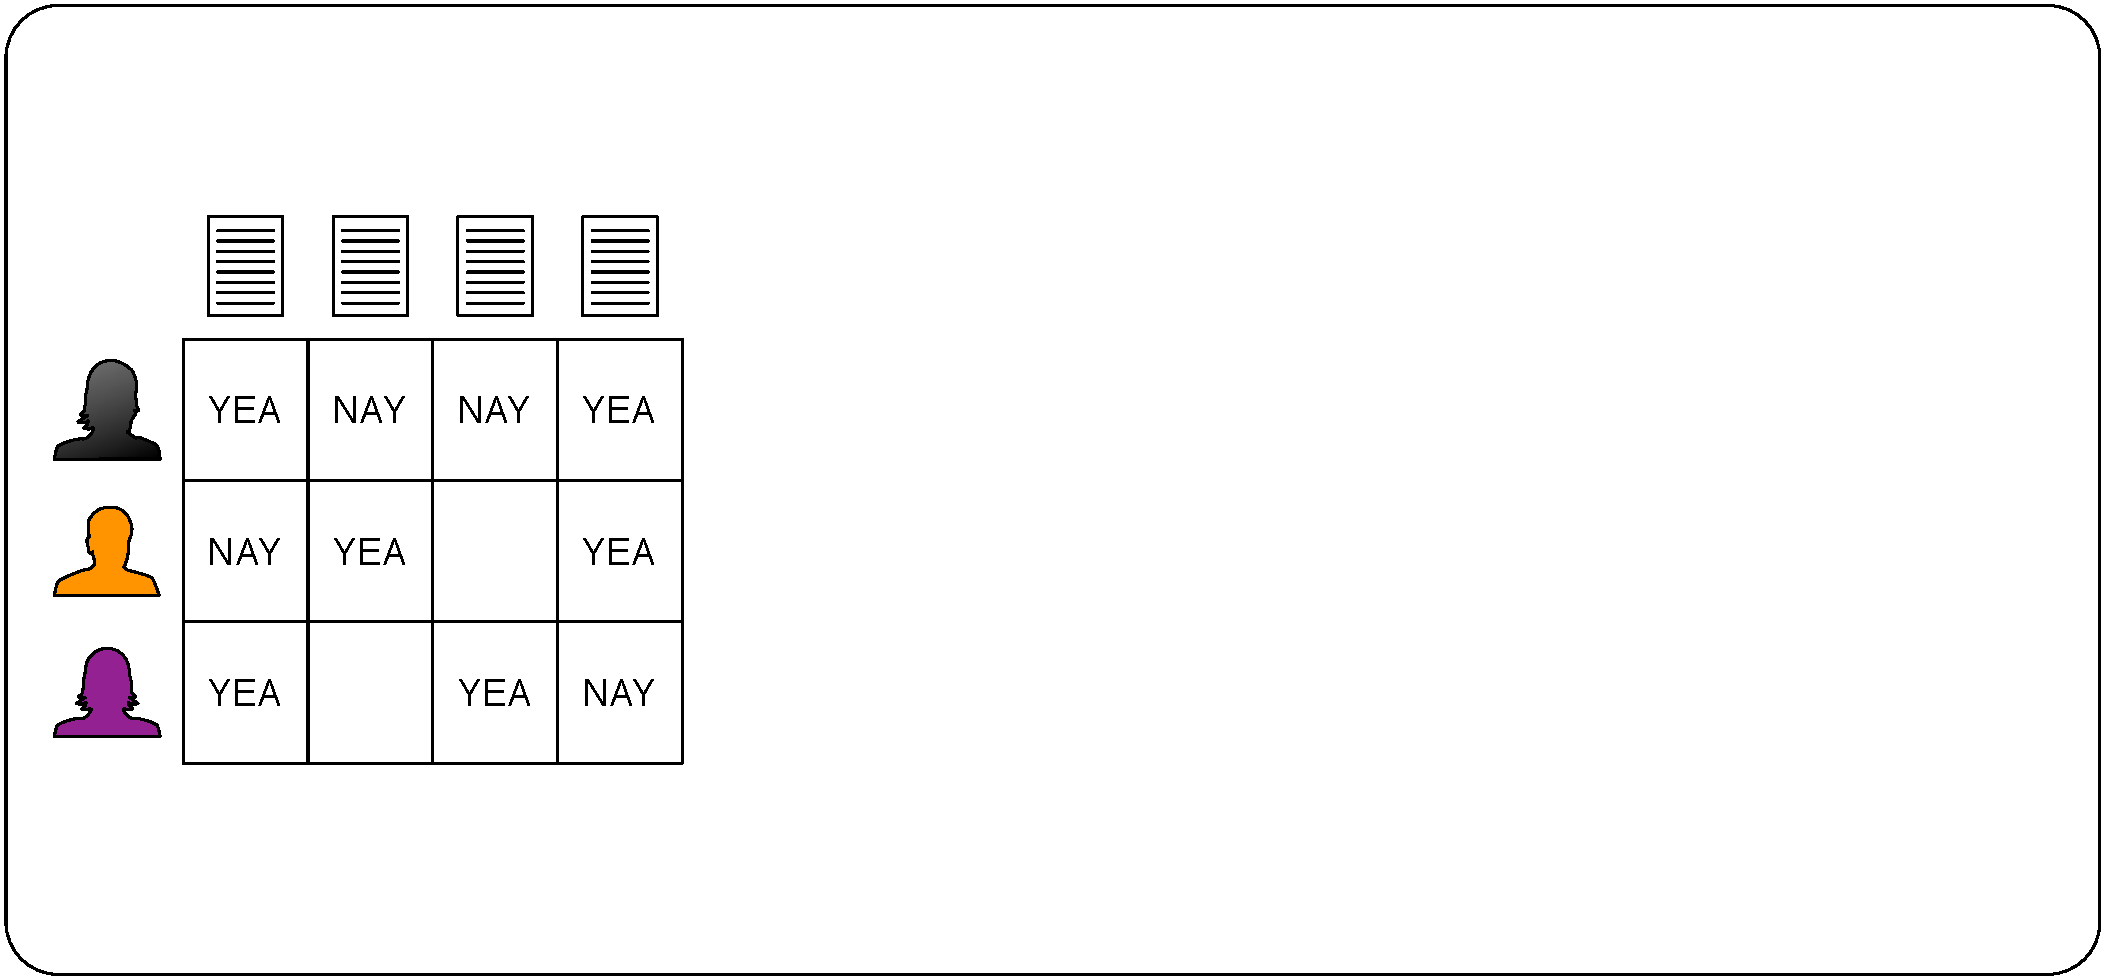
\includegraphics[width=.9\textwidth]{teaparty/figures/s5/1_votes}}%
        \only<2>{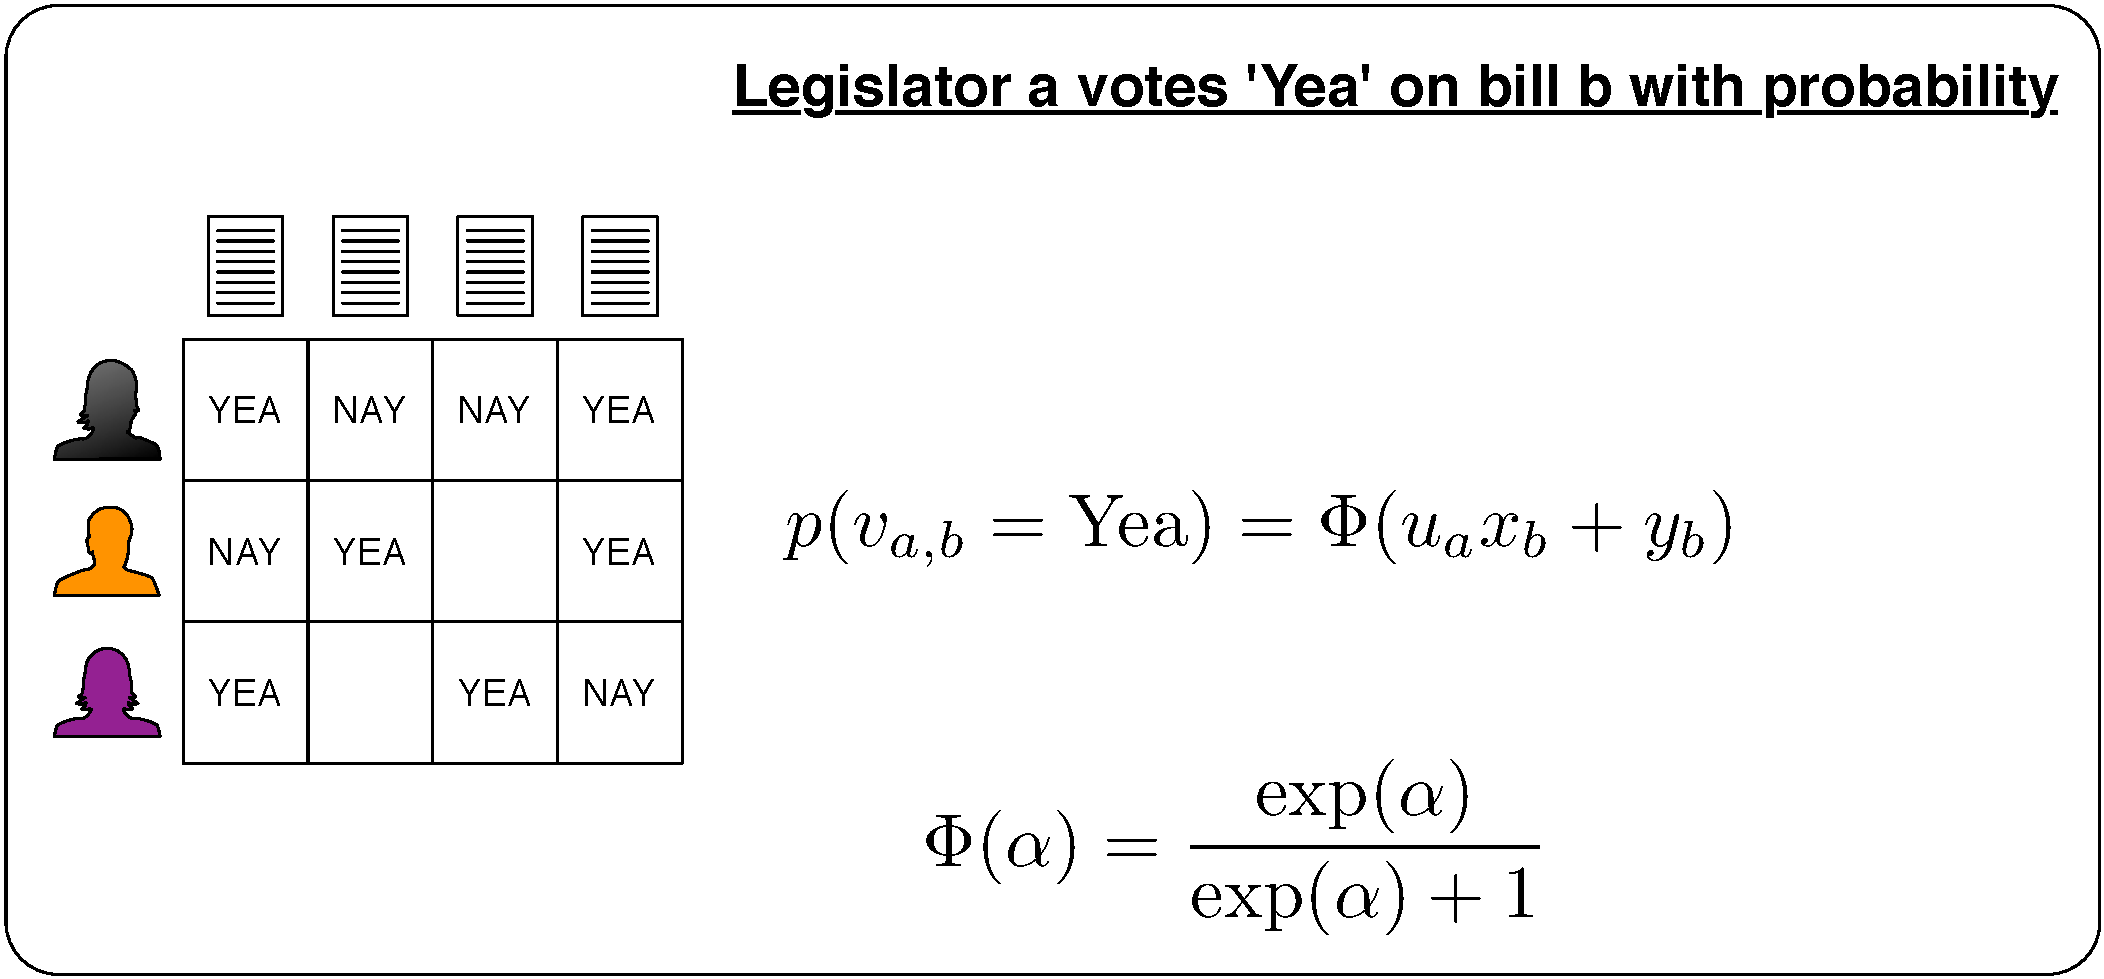
\includegraphics[width=.9\textwidth]{teaparty/figures/s5/2_onedim_ip_eqn}}%
        \only<3>{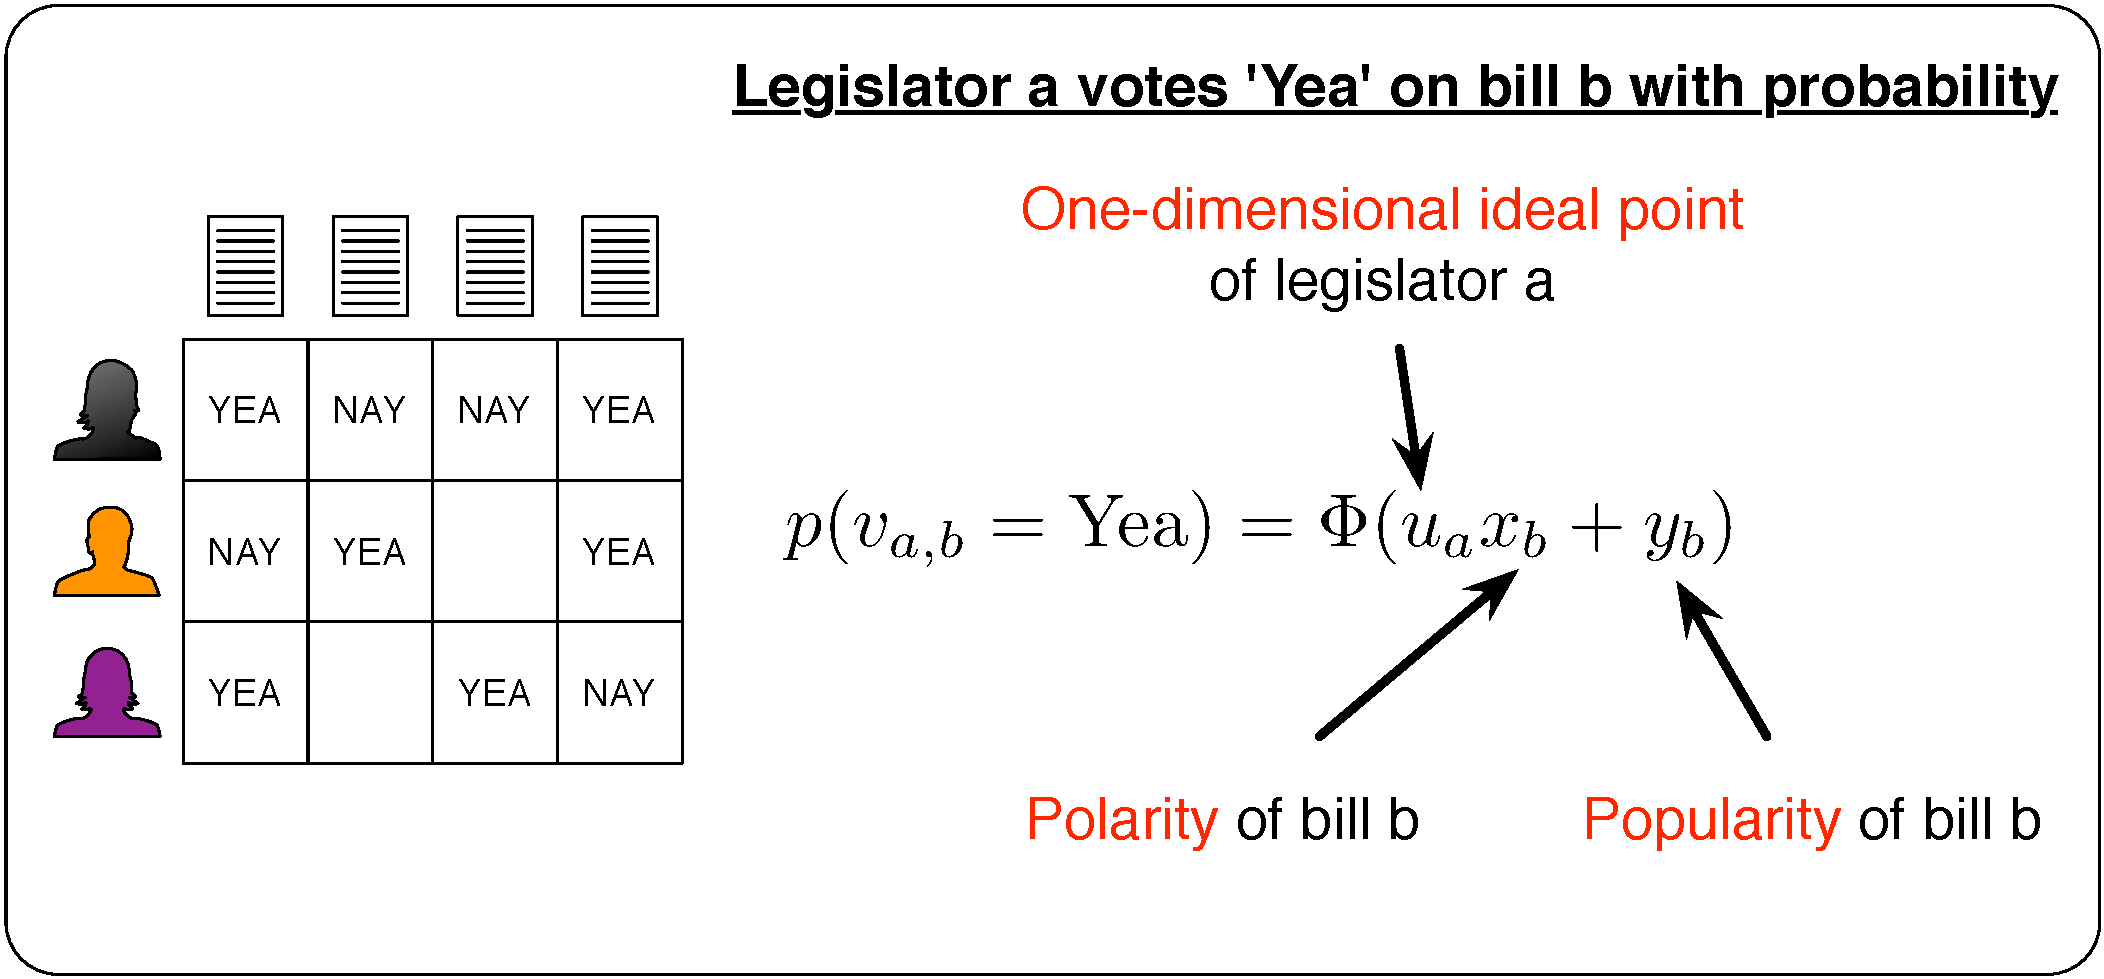
\includegraphics[width=.9\textwidth]{teaparty/figures/s5/3_onedim_ip_eqn_explained}}%
        \only<4->{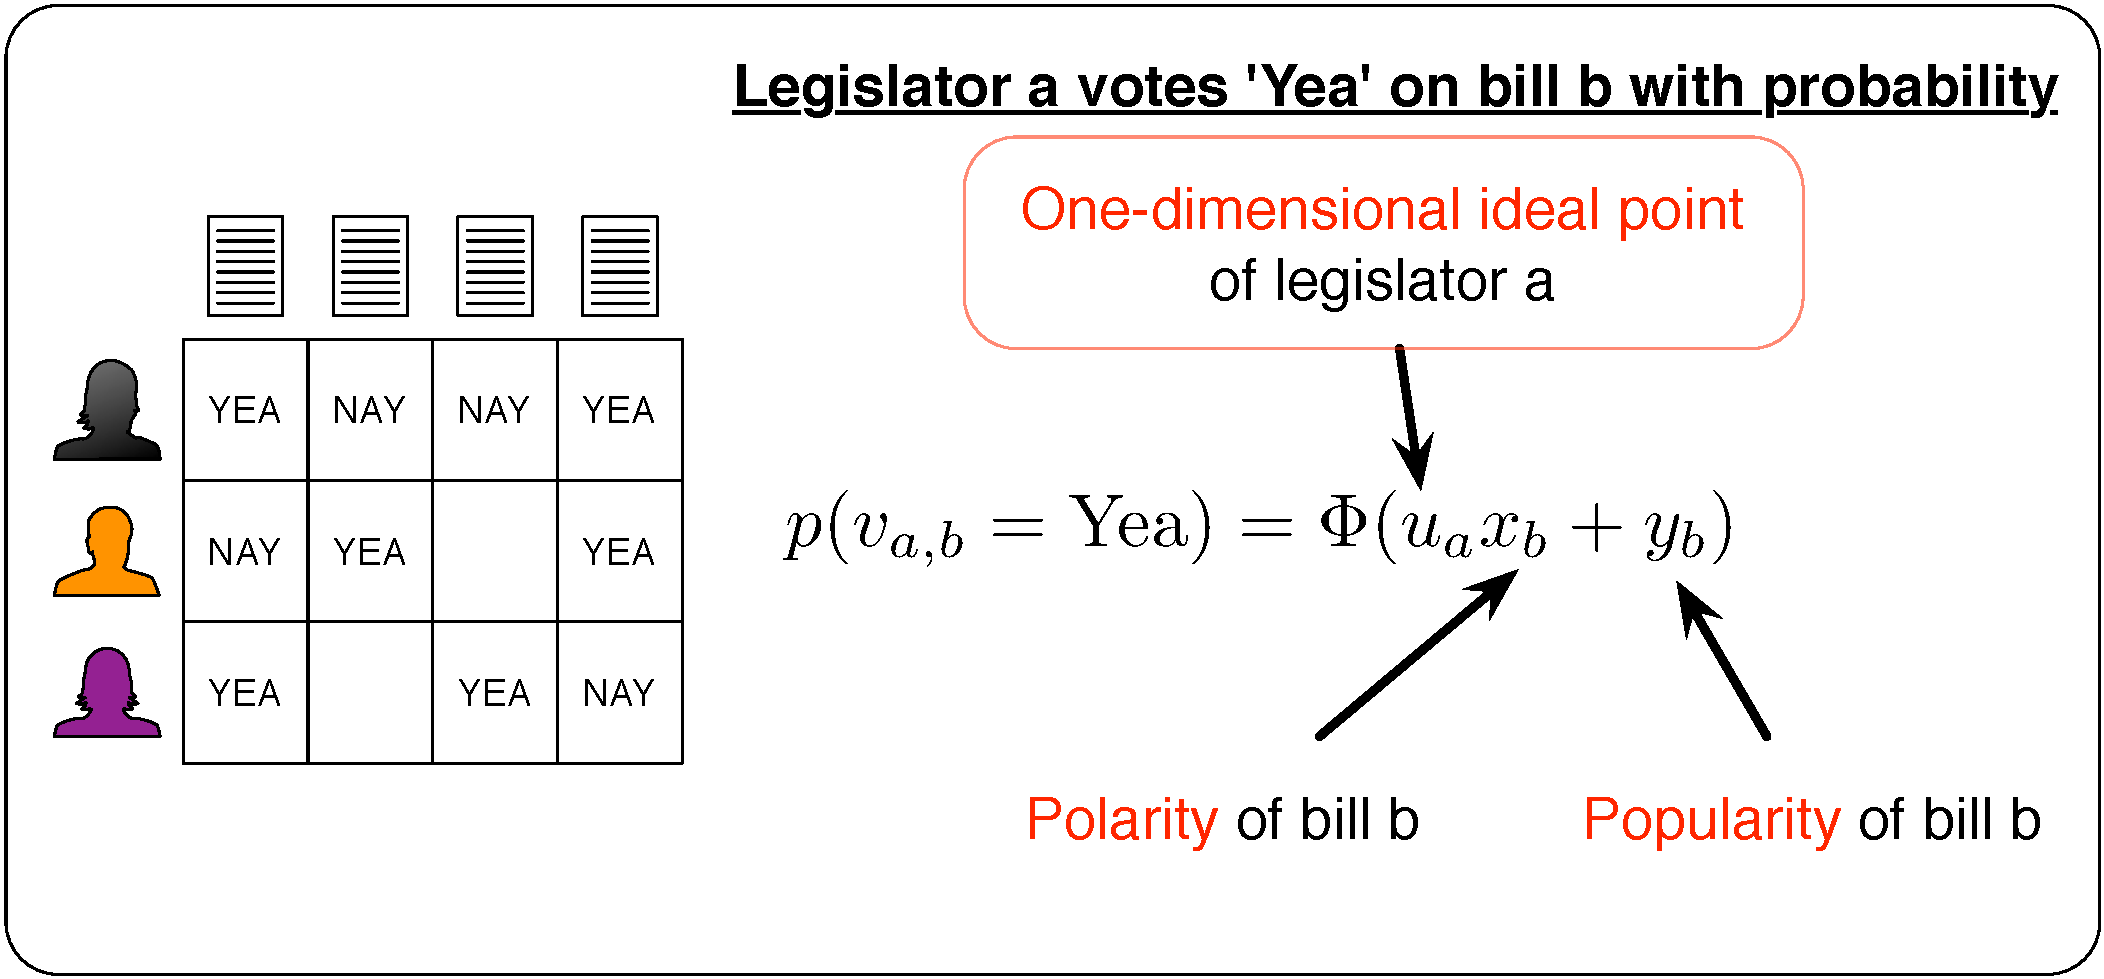
\includegraphics[width=.9\textwidth]{teaparty/figures/s5/3a_onedim_ip_eqn_highlighted}}%
    \end{figure}
    \vspace{-.3cm}
    \hfill \tiny{\cite{Poole:AJPS85}}

    \vspace{-0.5cm}

    \begin{columns}
      \column{\textwidth}
        \begin{center}
            \only<1-3>{
\includegraphics[width=.8\textwidth]{teaparty/figures/s5/dimensions_0}}%
            \only<4>{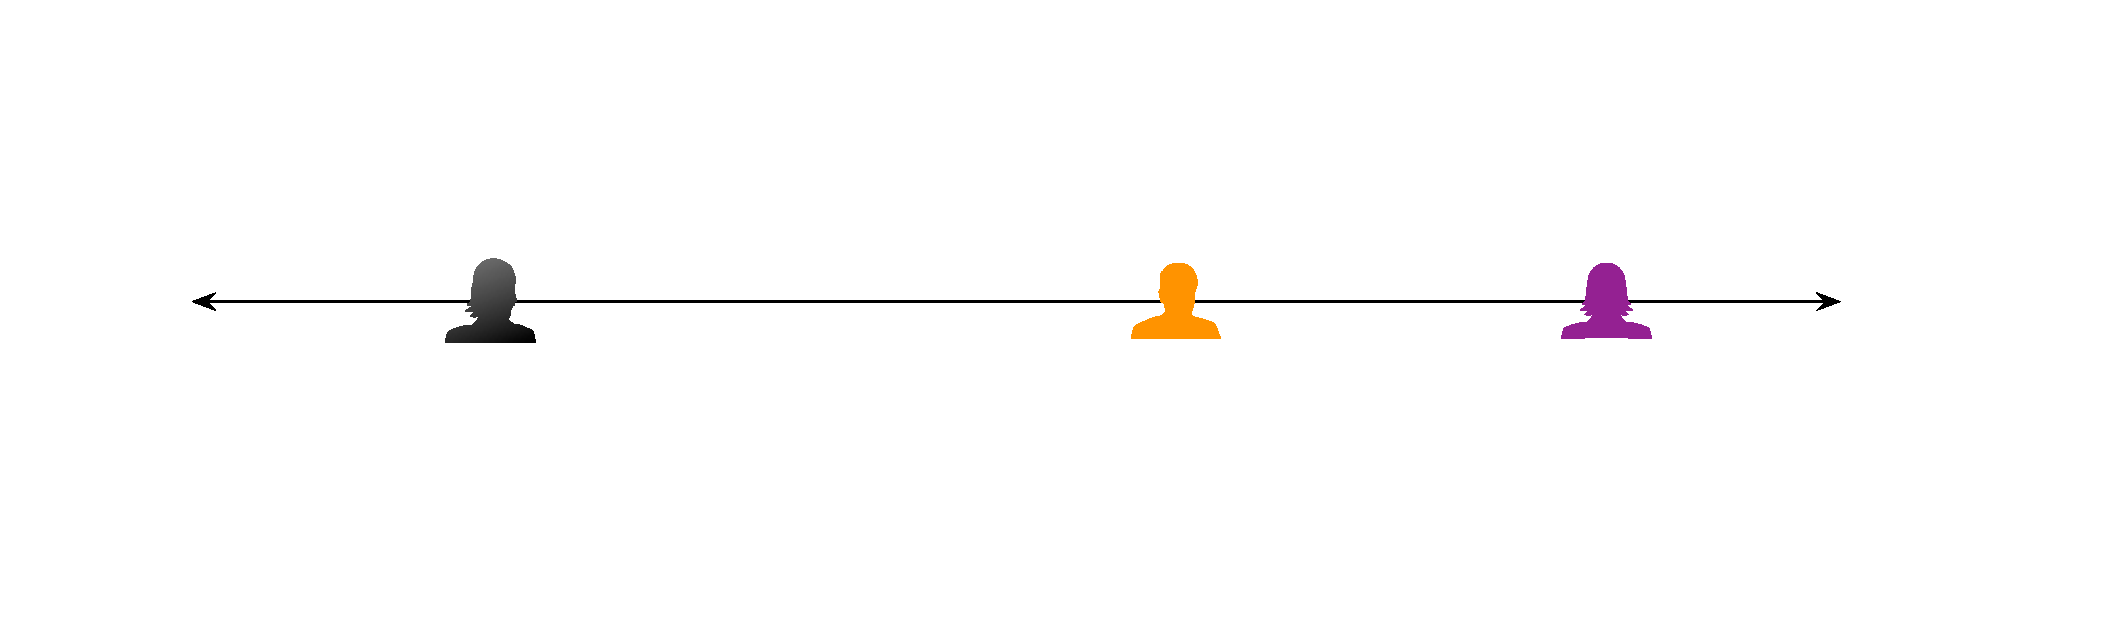
\includegraphics[width=.8\textwidth]{teaparty/figures/s5/dimensions_1}}%
            \only<5>{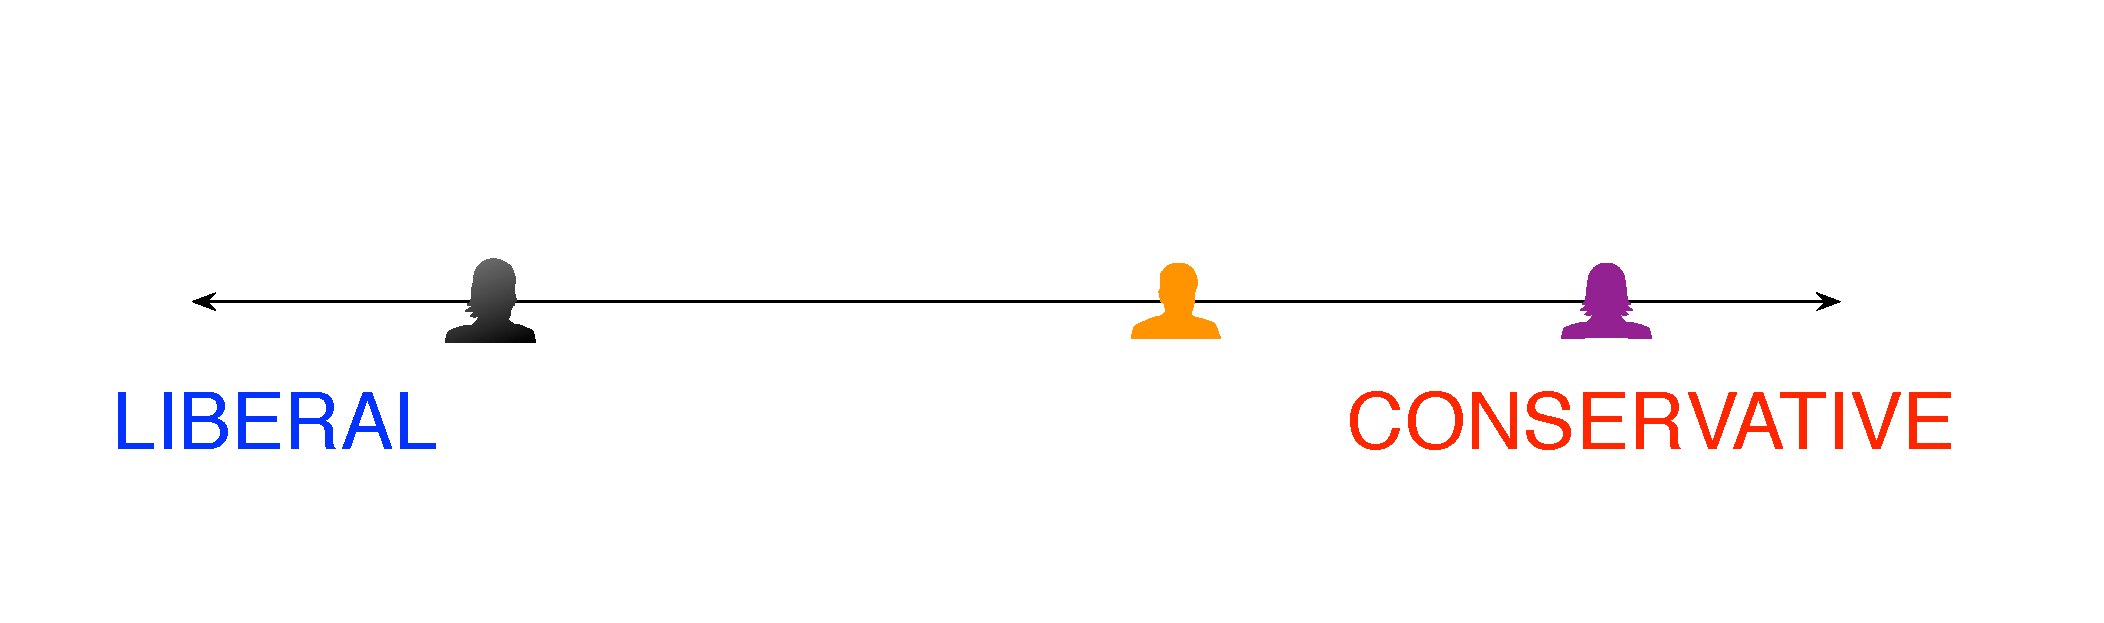
\includegraphics[width=.8\textwidth]{teaparty/figures/s5/dimensions_2}}%
        \end{center}
    \end{columns}
}%

\frame{
    \frametitle{Multi-dimensional Ideal Point using Votes}
    \begin{figure}
      \centering
        \only<1>{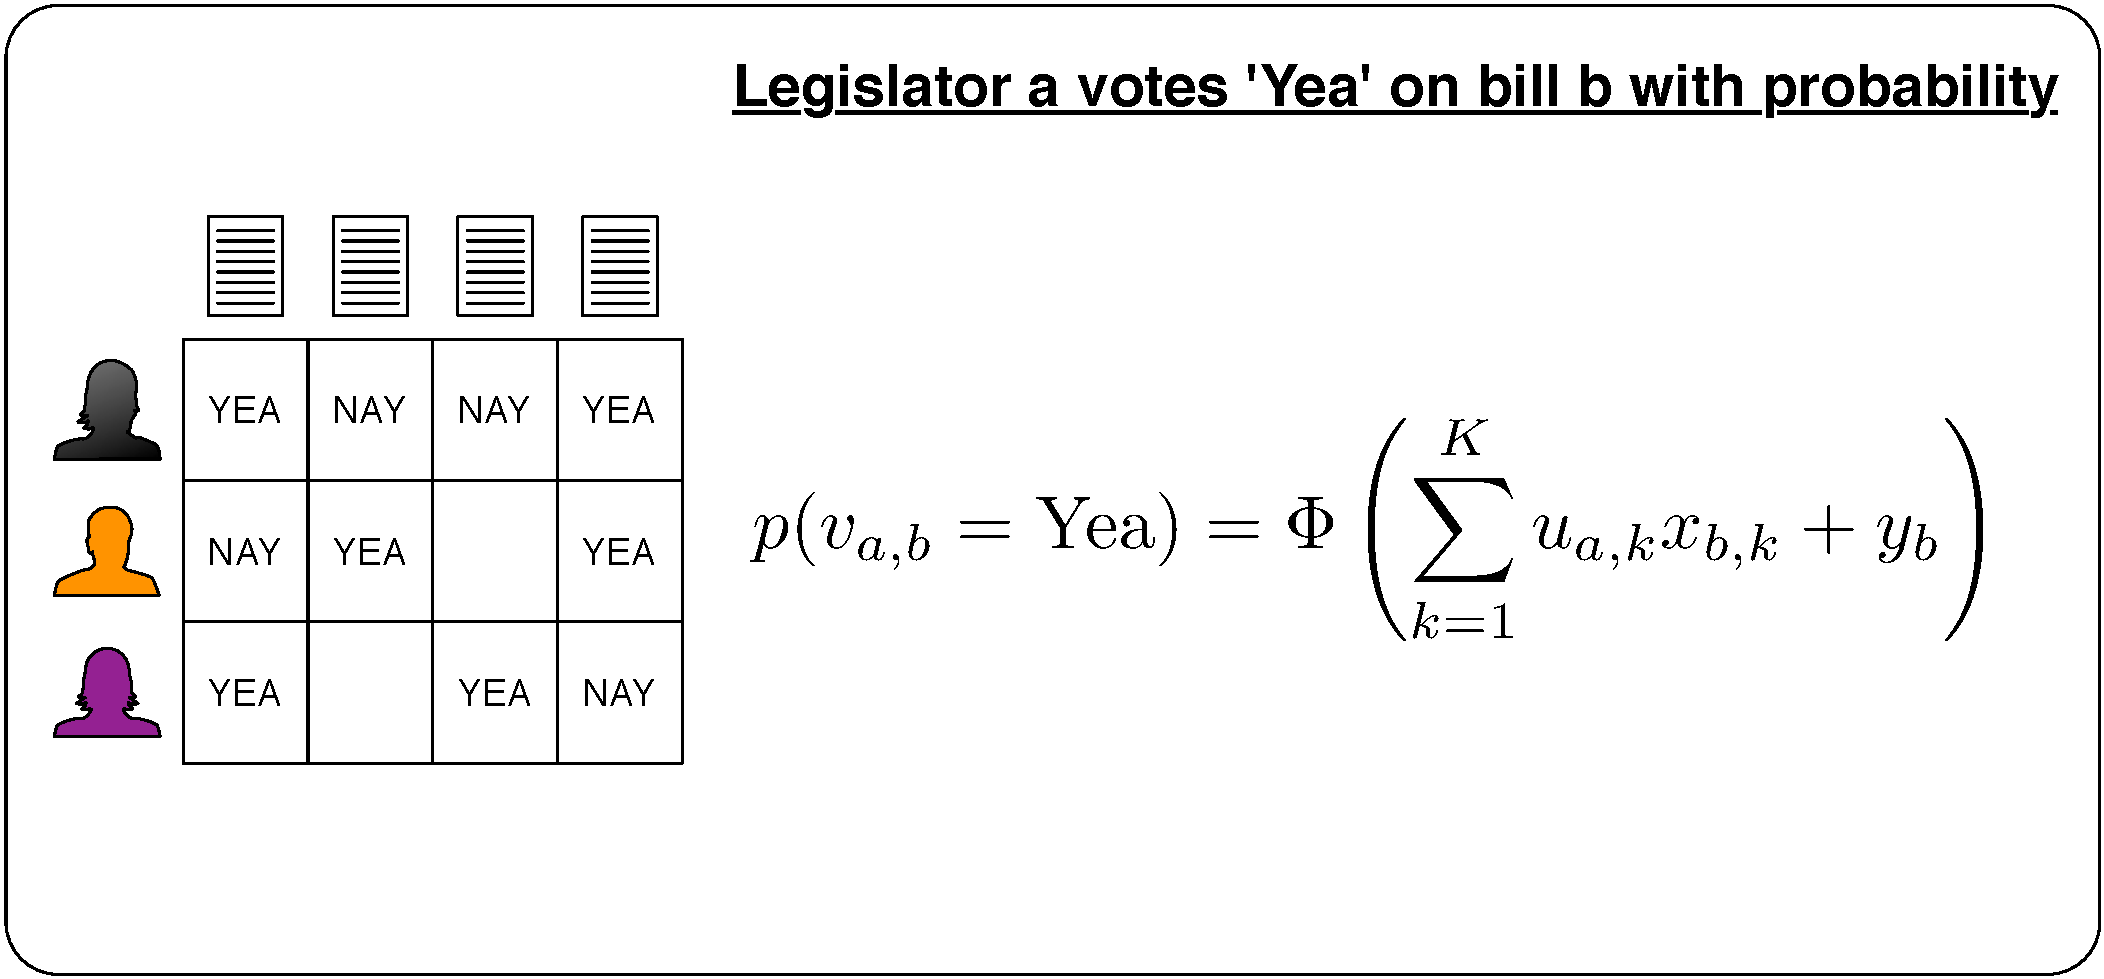
\includegraphics[width=.8\textwidth]{teaparty/figures/s5/4_multdim_ip_eqn}}%
        \only<2>{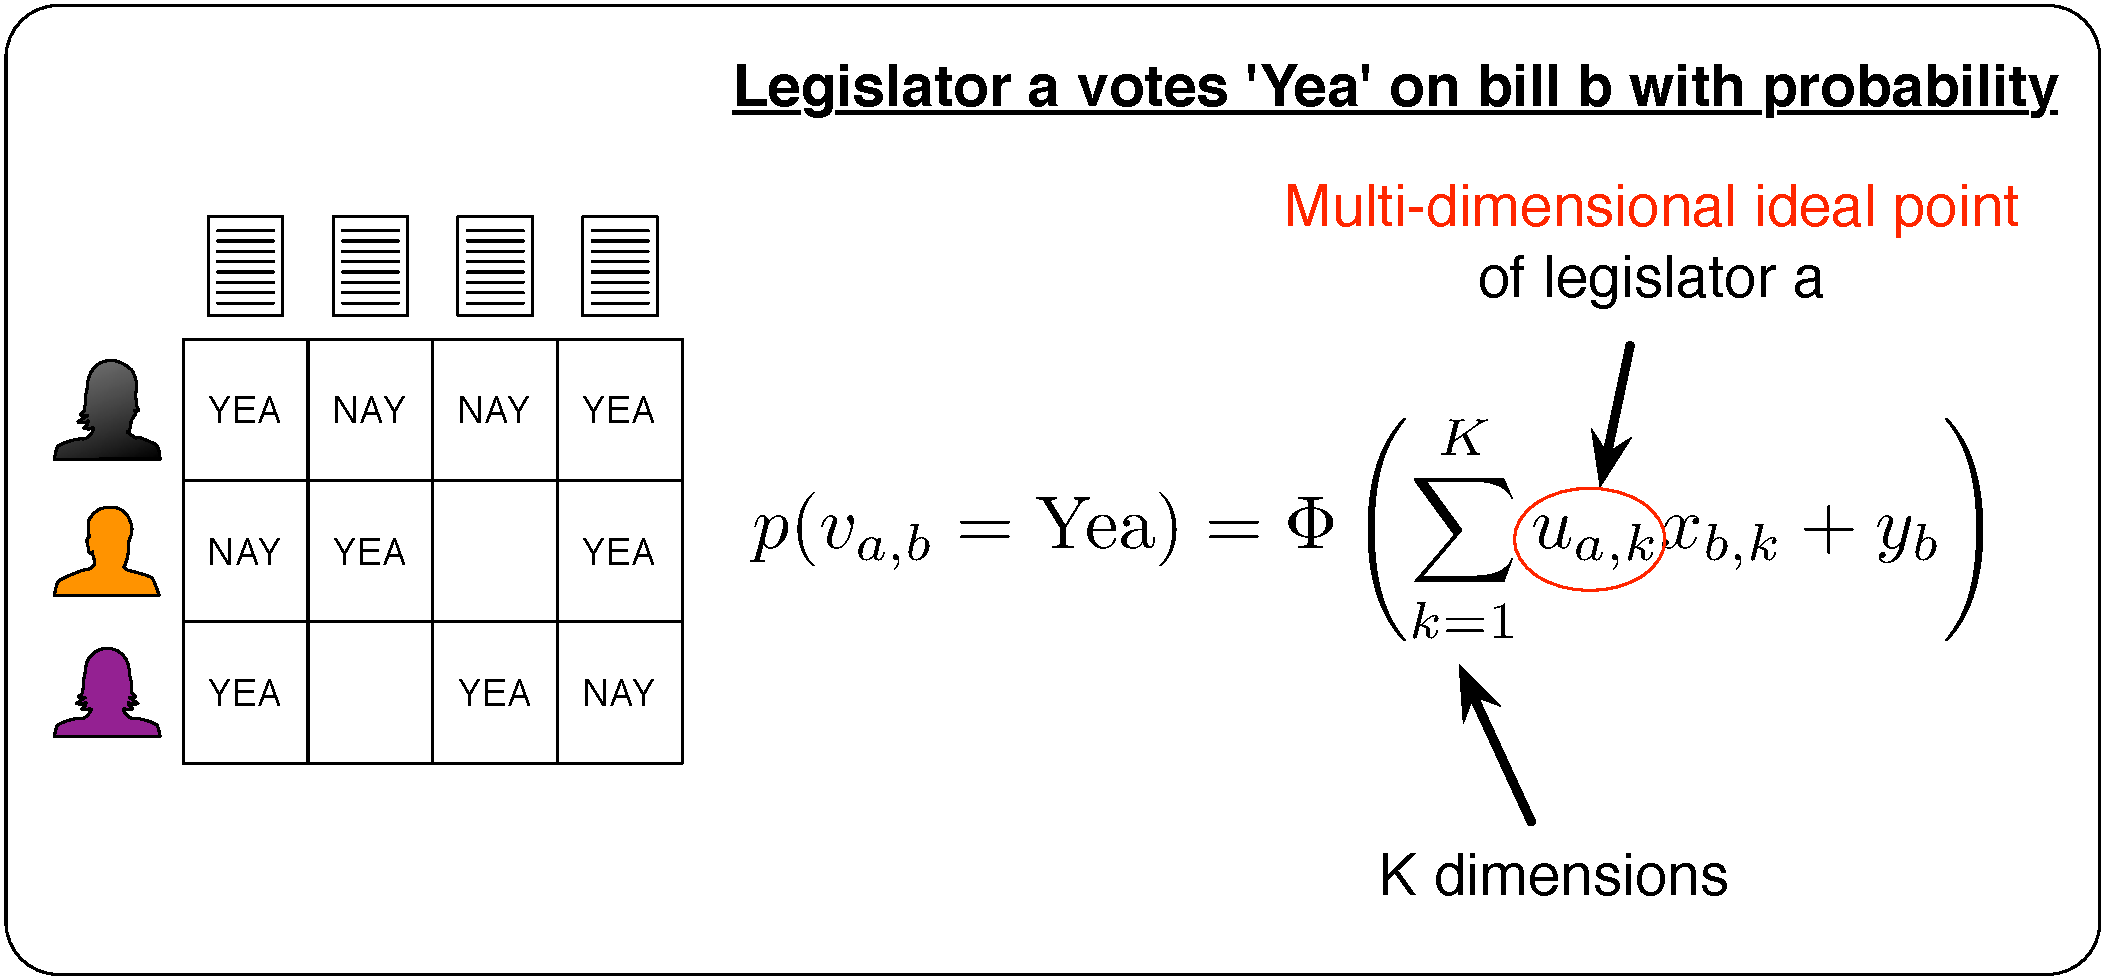
\includegraphics[width=.8\textwidth]{teaparty/figures/s5/5_multdim_ip_eqn_explained}}%
        \only<3->{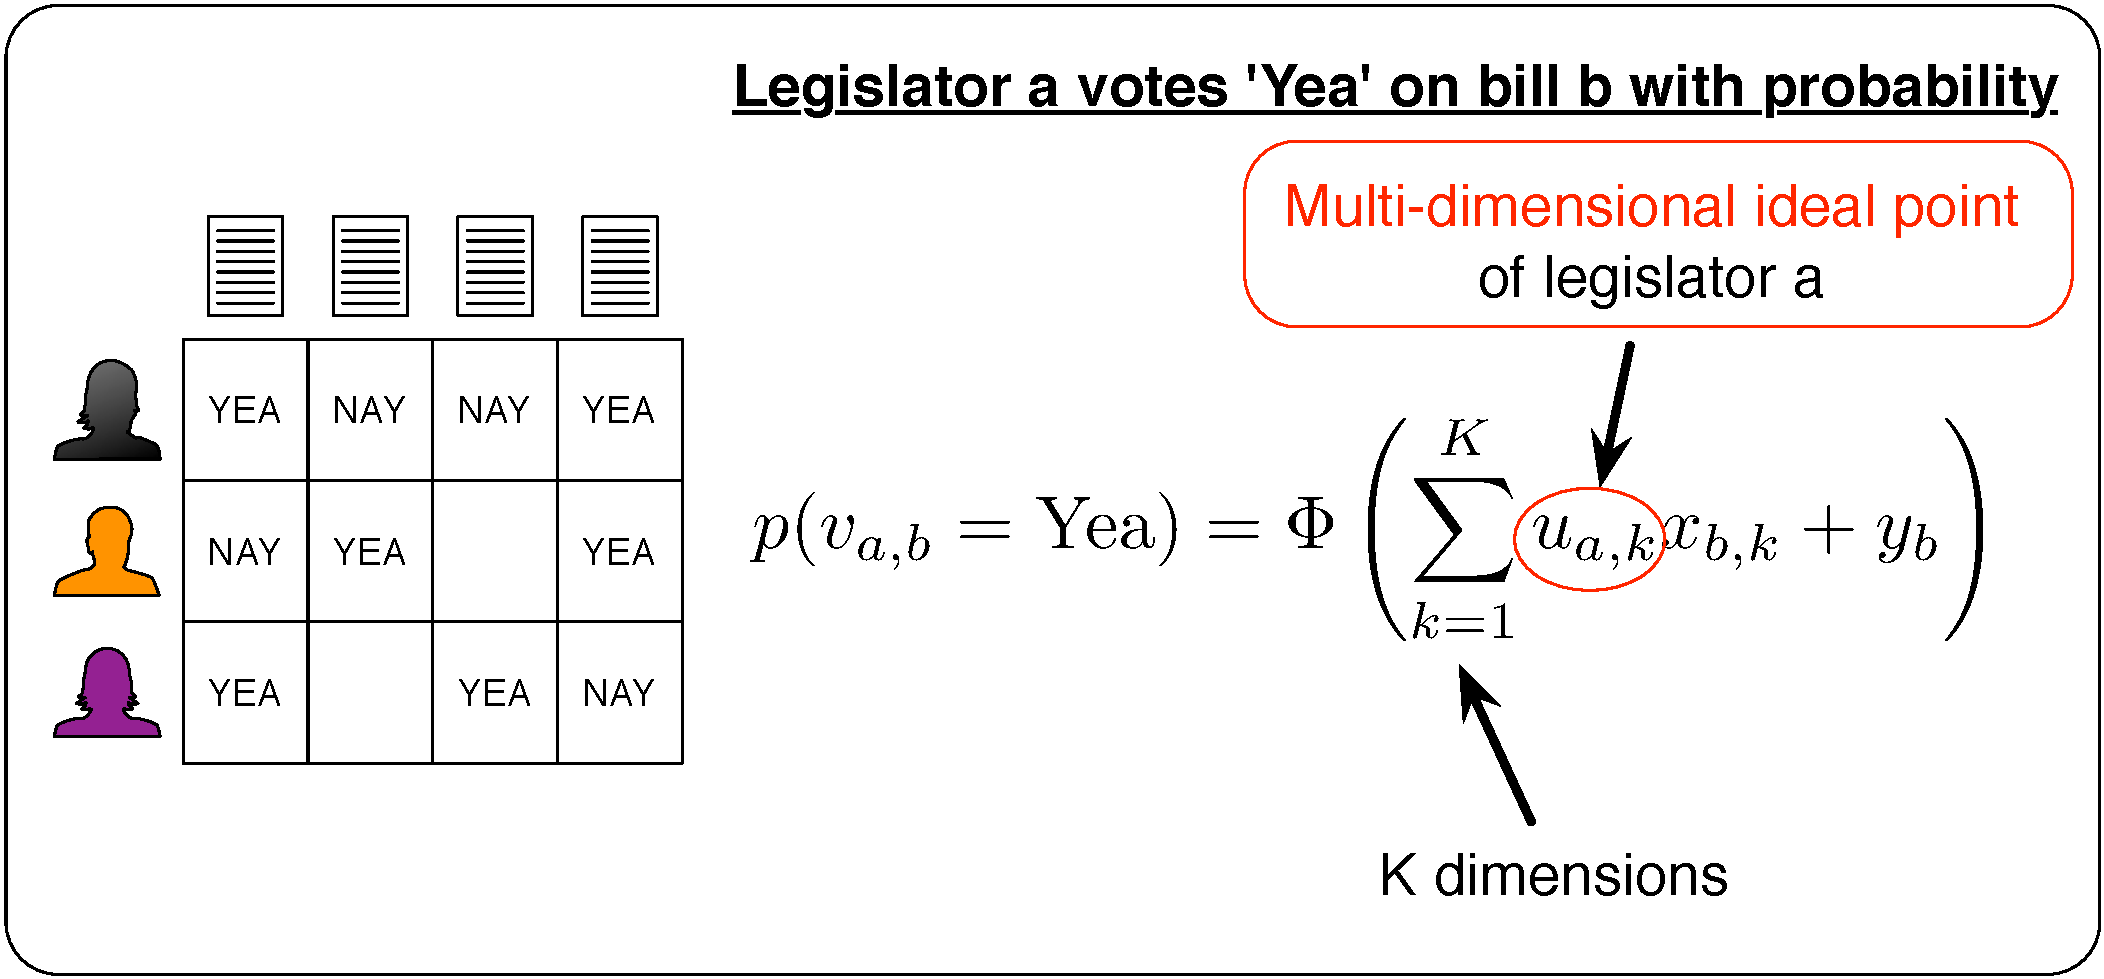
\includegraphics[width=.8\textwidth]{teaparty/figures/s5/5a_multdim_ip_eqn_highlighted}}%
    \end{figure}
    \vspace{-.2cm}    
    \hfill \tiny{\cite{Heckman:NBER96,Jackman:PA01,Clinton:APSR04}}    
    \vspace{-.3cm}
    \begin{figure}
        \only<1-2>{
\includegraphics[width=.7\textwidth]{teaparty/figures/s5/dimensions_0}}%
        \only<3>{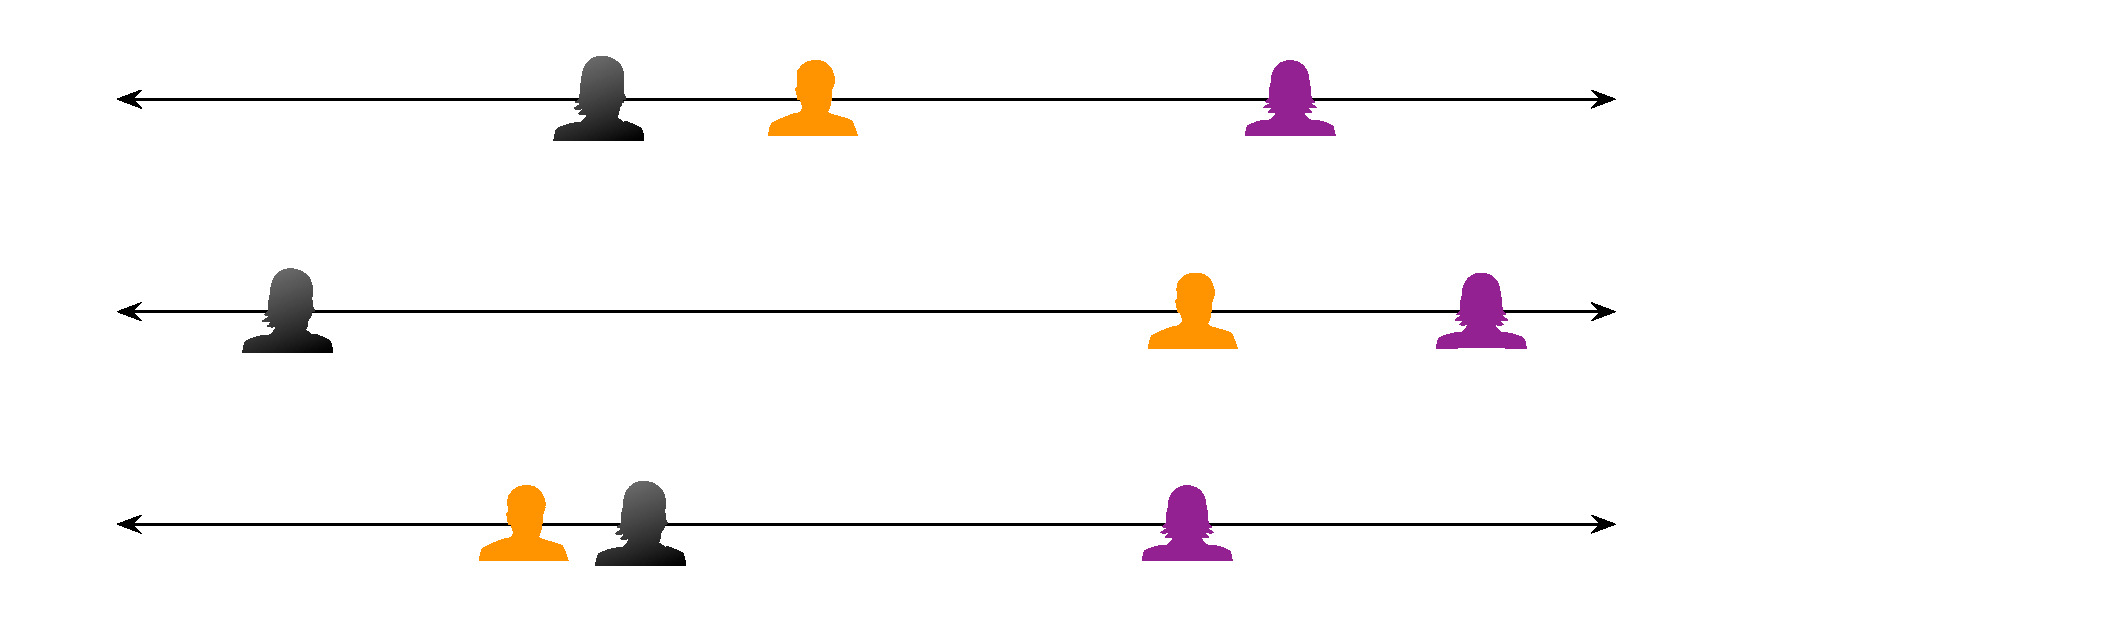
\includegraphics[width=.7\textwidth]{teaparty/figures/s5/dimensions_3}}%
        \only<4>{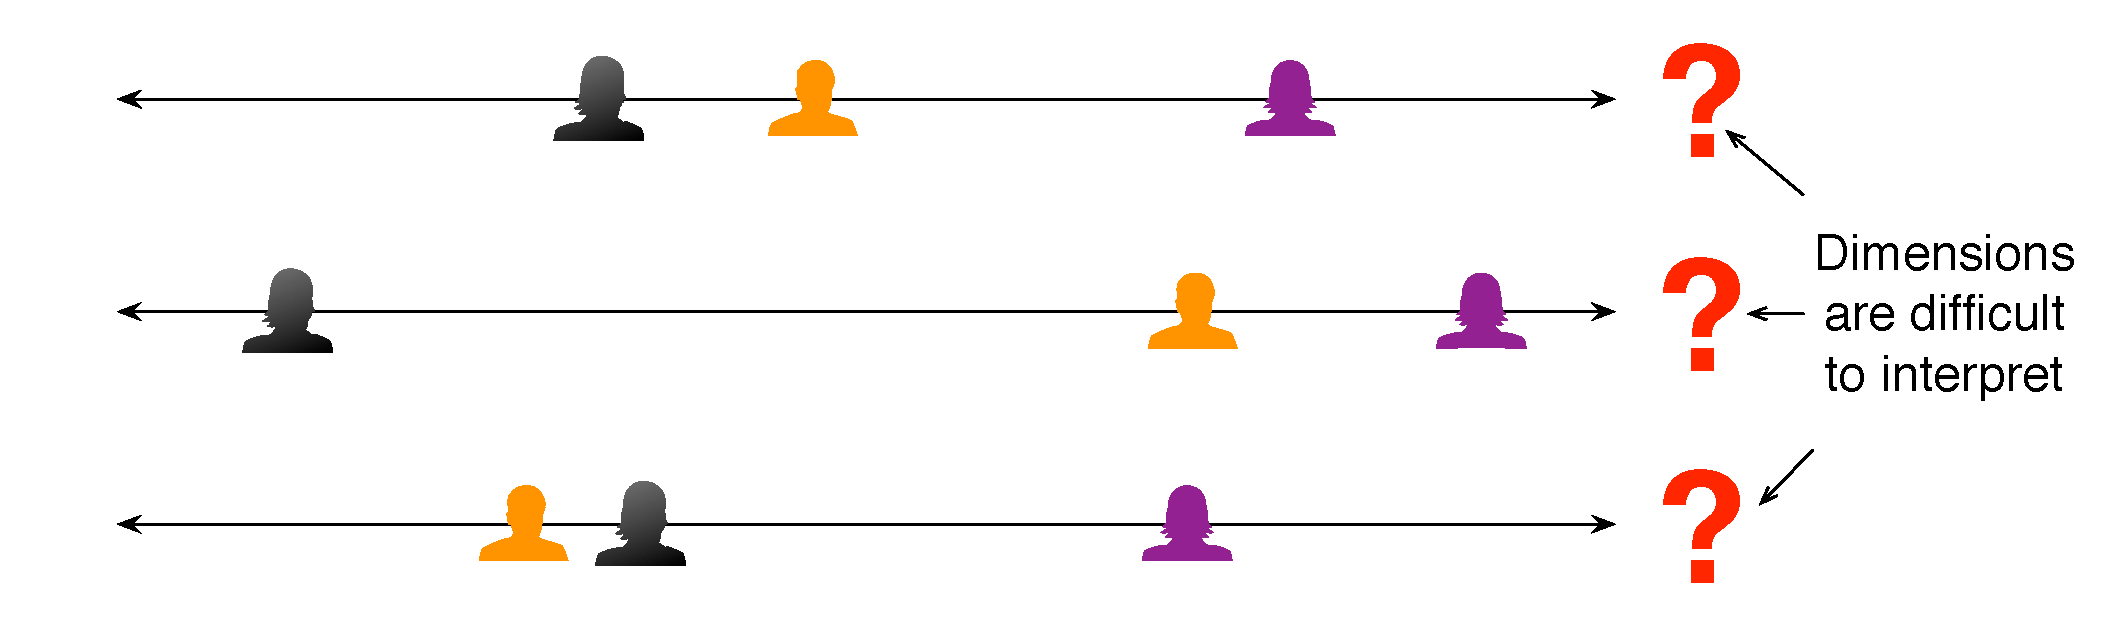
\includegraphics[width=.7\textwidth]{teaparty/figures/s5/dimensions_4}}%
    \end{figure}
}%

\frame{
    \frametitle{Multi-dimensional Ideal Point using Votes \& \textbf{Text}}
    \begin{figure}
      \centering
        \only<1>{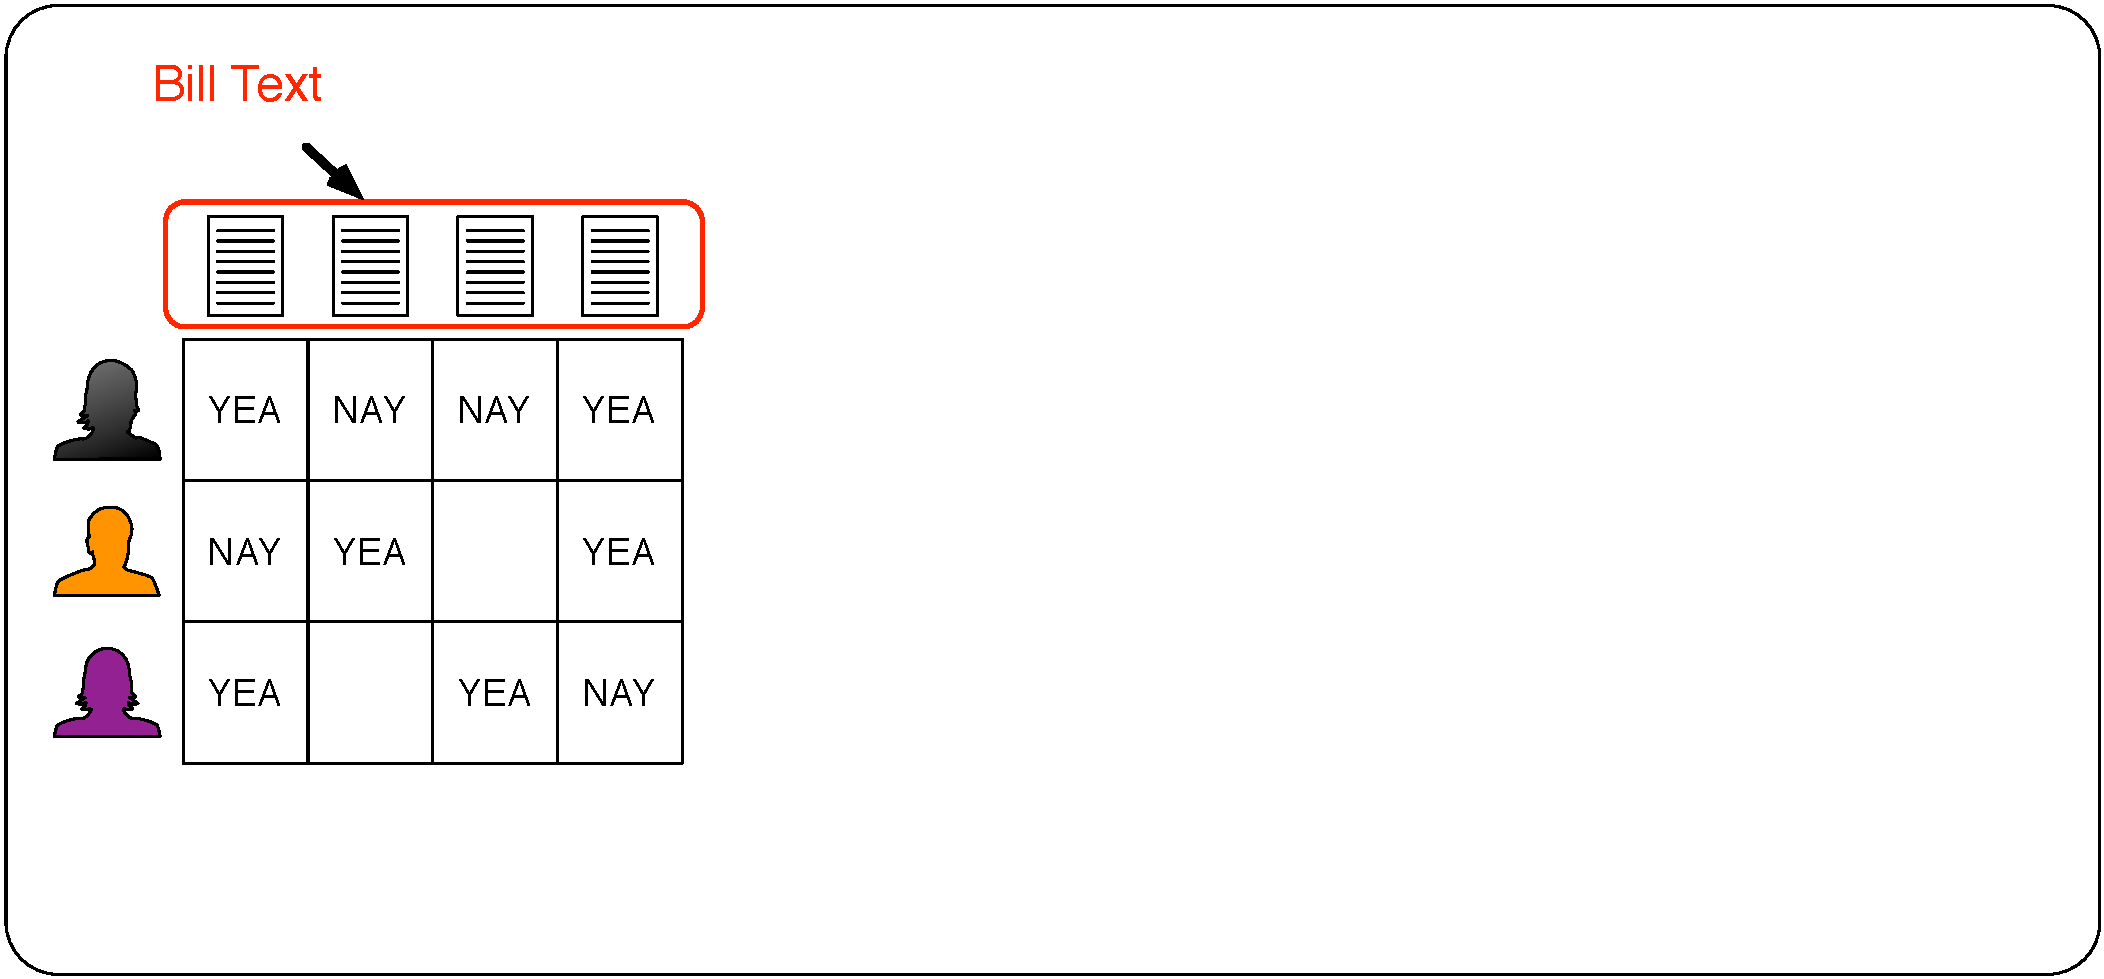
\includegraphics[width=.8\textwidth]{teaparty/figures/s5/1a_votes_text}}%
        \only<2>{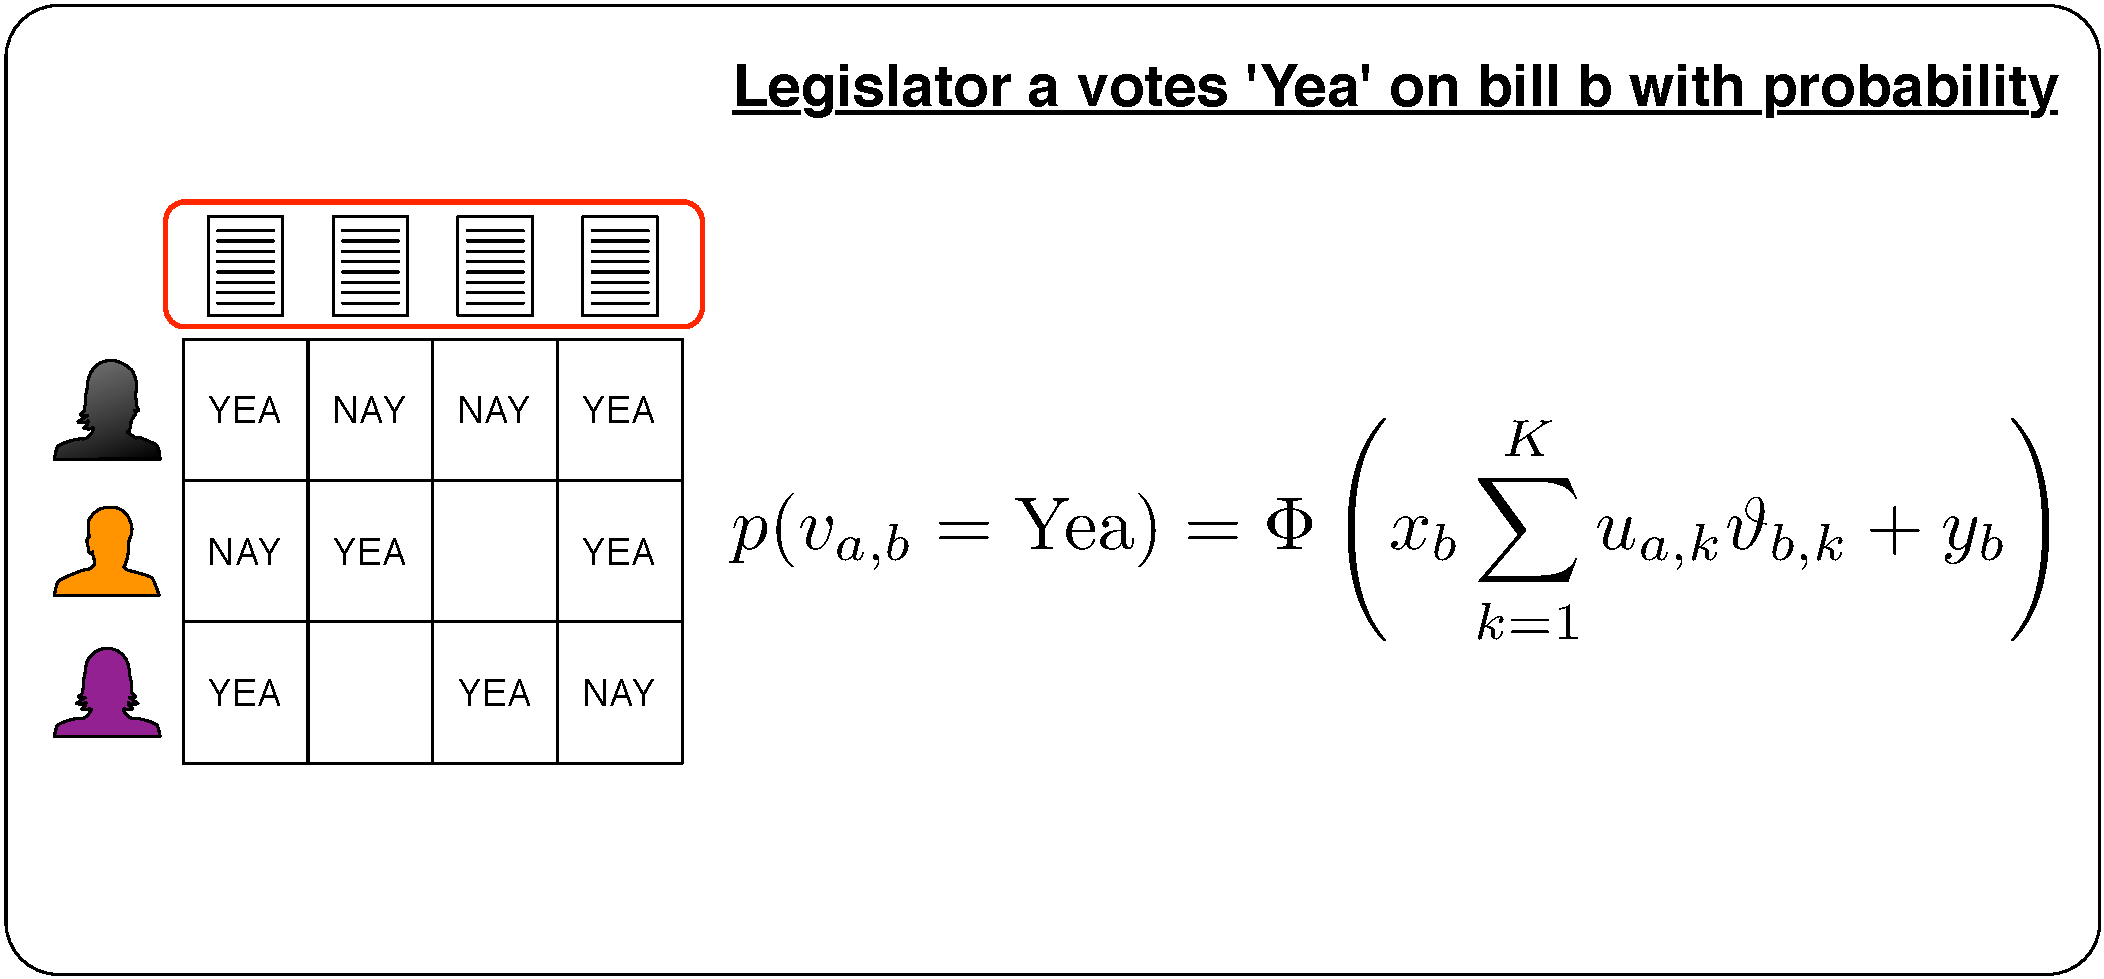
\includegraphics[width=.8\textwidth]{teaparty/figures/s5/6_multdim_ip_text_eqn}}%
        \only<3->{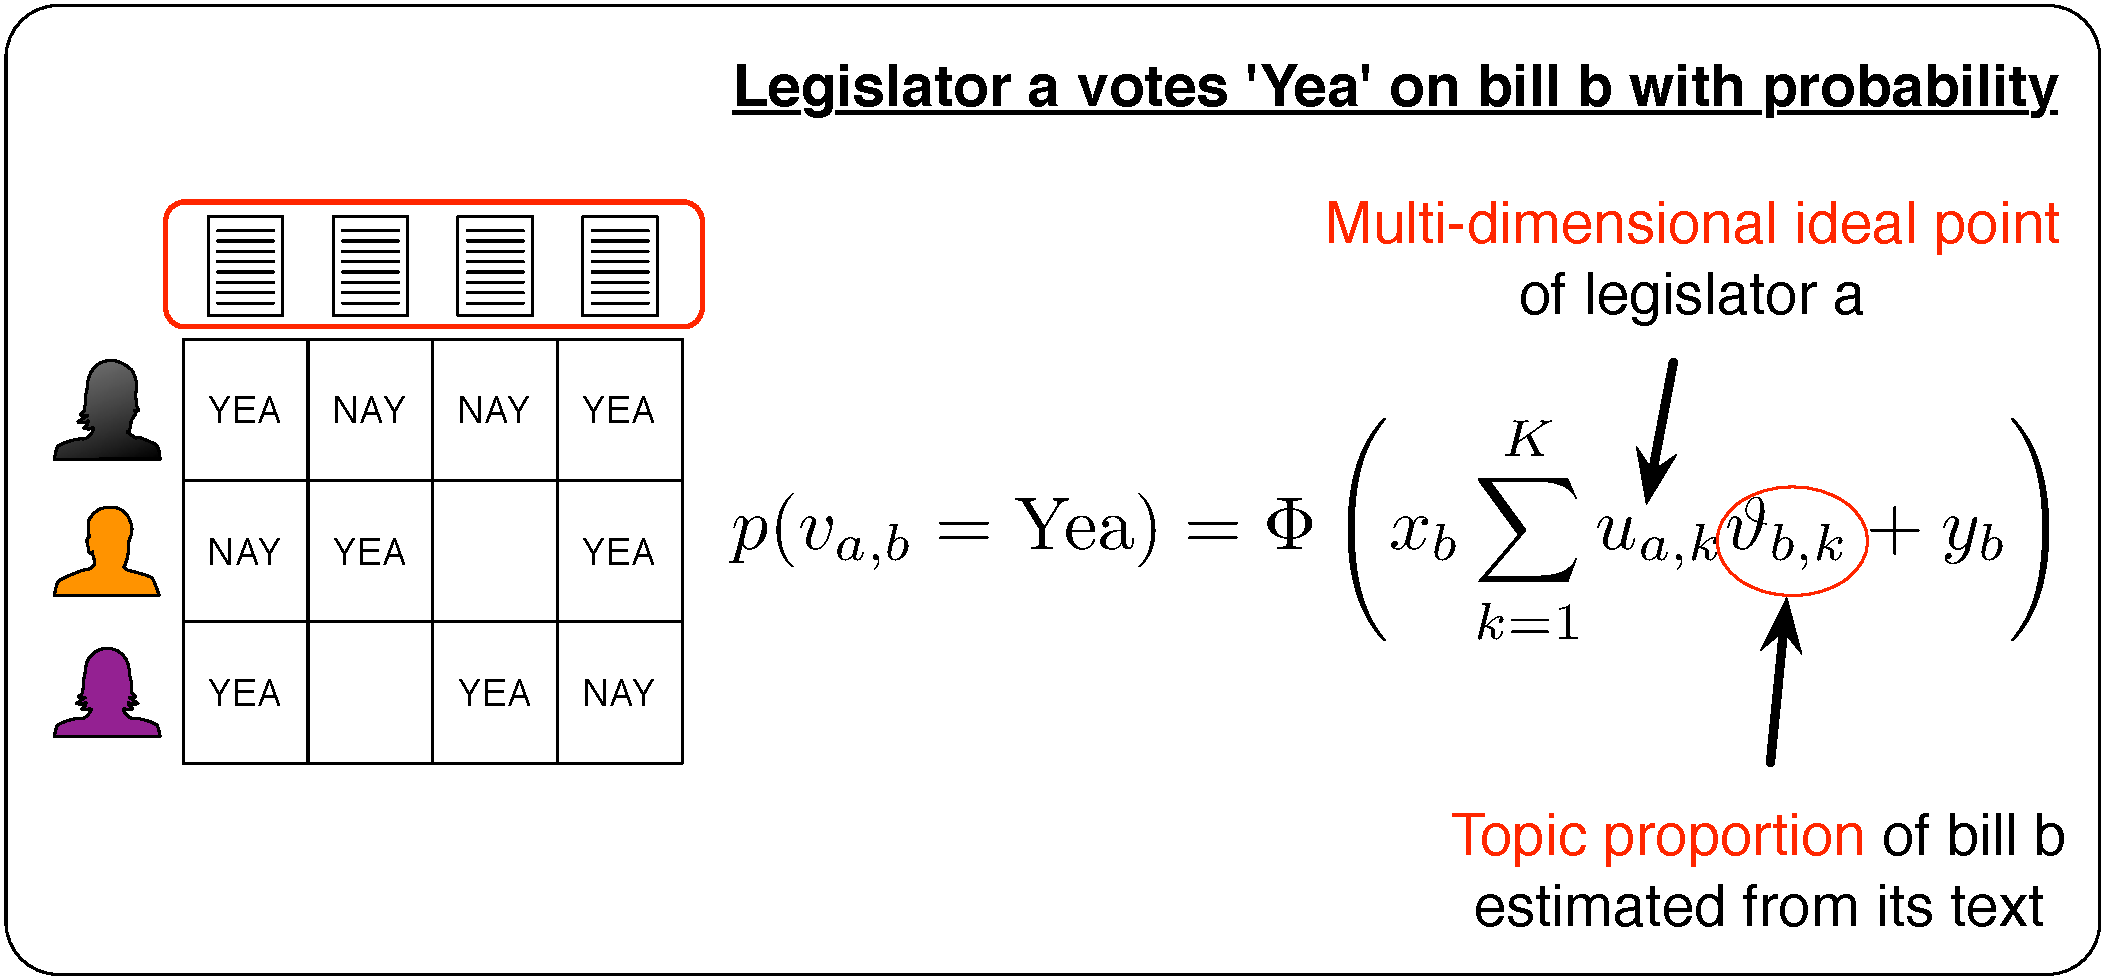
\includegraphics[width=.8\textwidth]{teaparty/figures/s5/7_multdim_ip_text_eqn_explained}}%
    \end{figure}
    \vspace{-.3cm}
    \hfill \tiny{} \cite{Gerrish:NIPS12,Bonica:AJPS13:ideology,Lauderdale:AJPS14,Sim:AAAI15:utility}
    \begin{figure}
        \only<1-3>{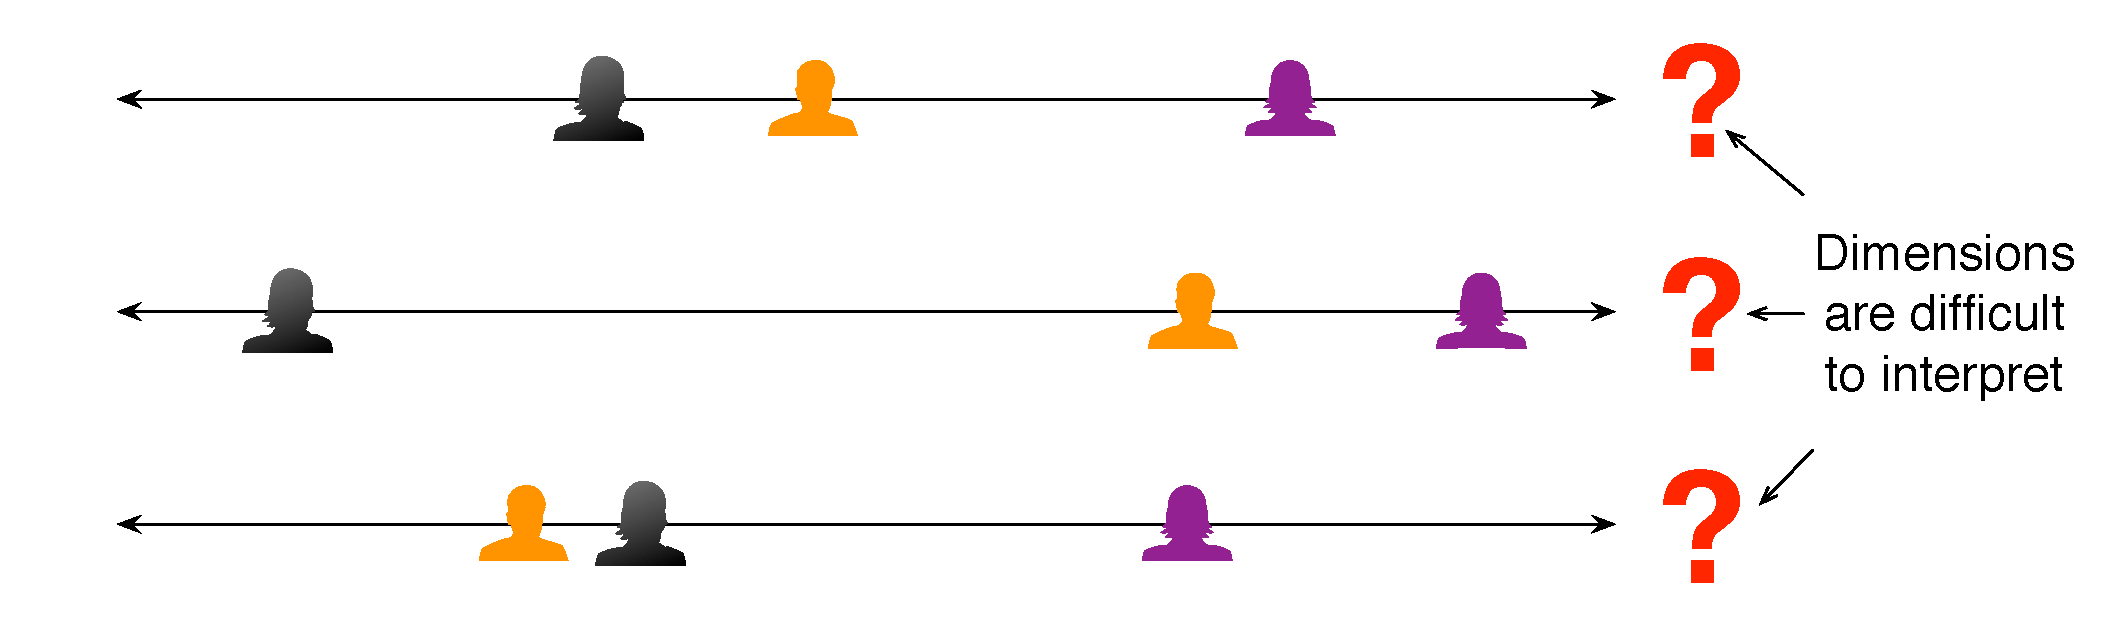
\includegraphics[width=.7\textwidth]{teaparty/figures/s5/dimensions_4}}%
        \only<4->{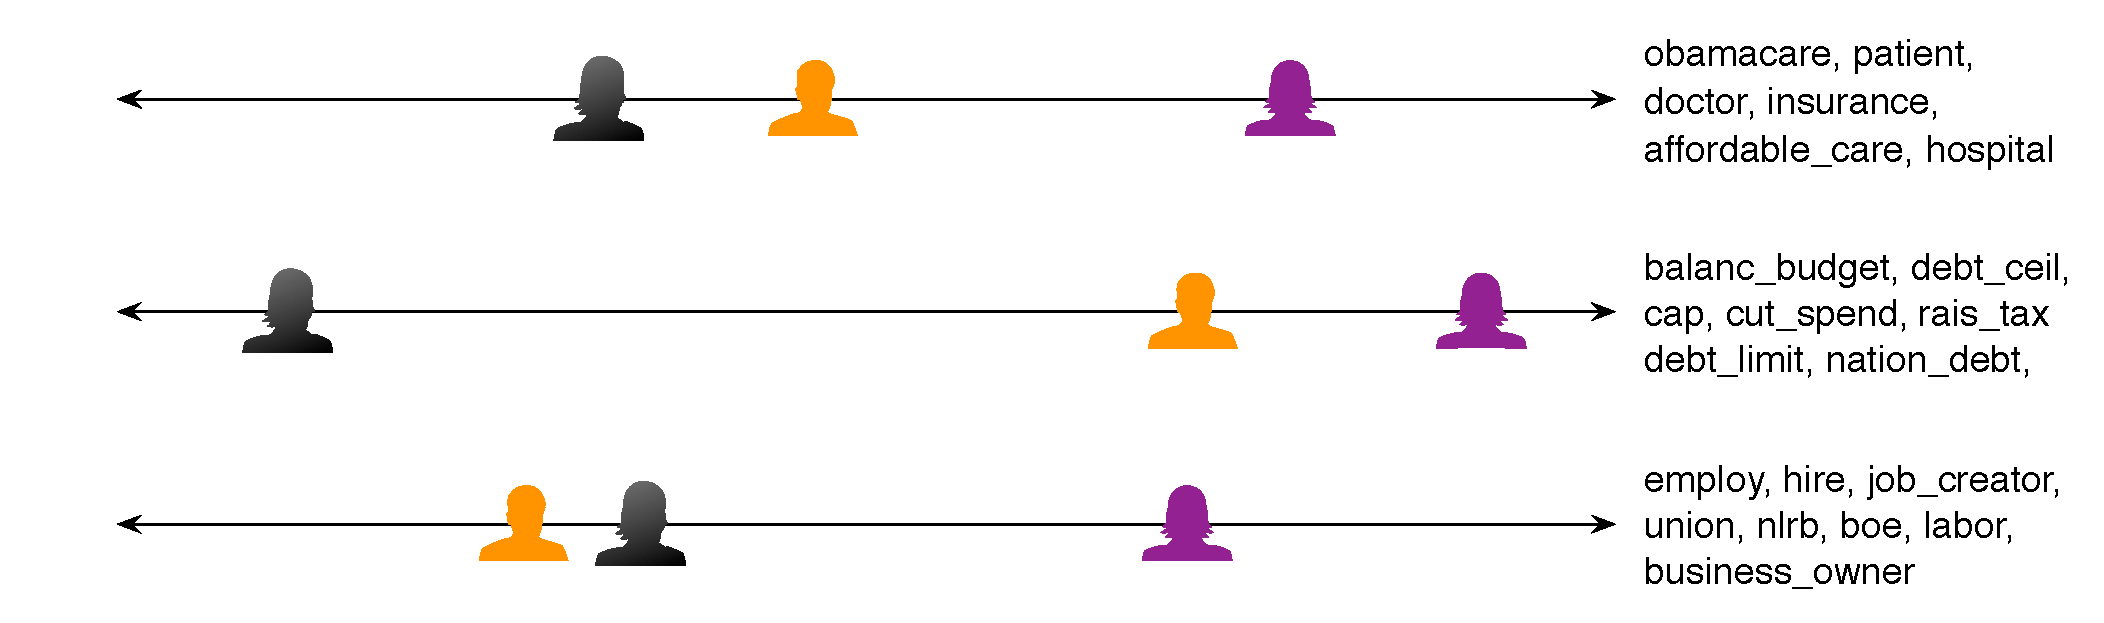
\includegraphics[width=.7\textwidth]{teaparty/figures/s5/dimensions_5}}%
    \end{figure}
}%

\begin{frame}{First-level topics from Political Scientists}

\begin{columns}
	\column{.5\linewidth}
		\begin{itemize}
			\item Government 
			\item Trade
			\item Defense
			\item Law and Crime 
			\item Transportation 		
			\item Parks and Lands 										
		\end{itemize}
	\column{.5\linewidth}
		\begin{itemize}
			\item Energy 
			\item Environment 
			\item Education 
			\item Labor Issues 
			\item Health 
			\item Rights and Liberties 												
		\end{itemize}
	
\end{columns}

\end{frame}

\section{Hierarchical Ideal Point Topic Model}

\frame{
    \frametitle{Our approach: Hierarchical Ideal Point Topic Model}
    \begin{figure}
    \centering
      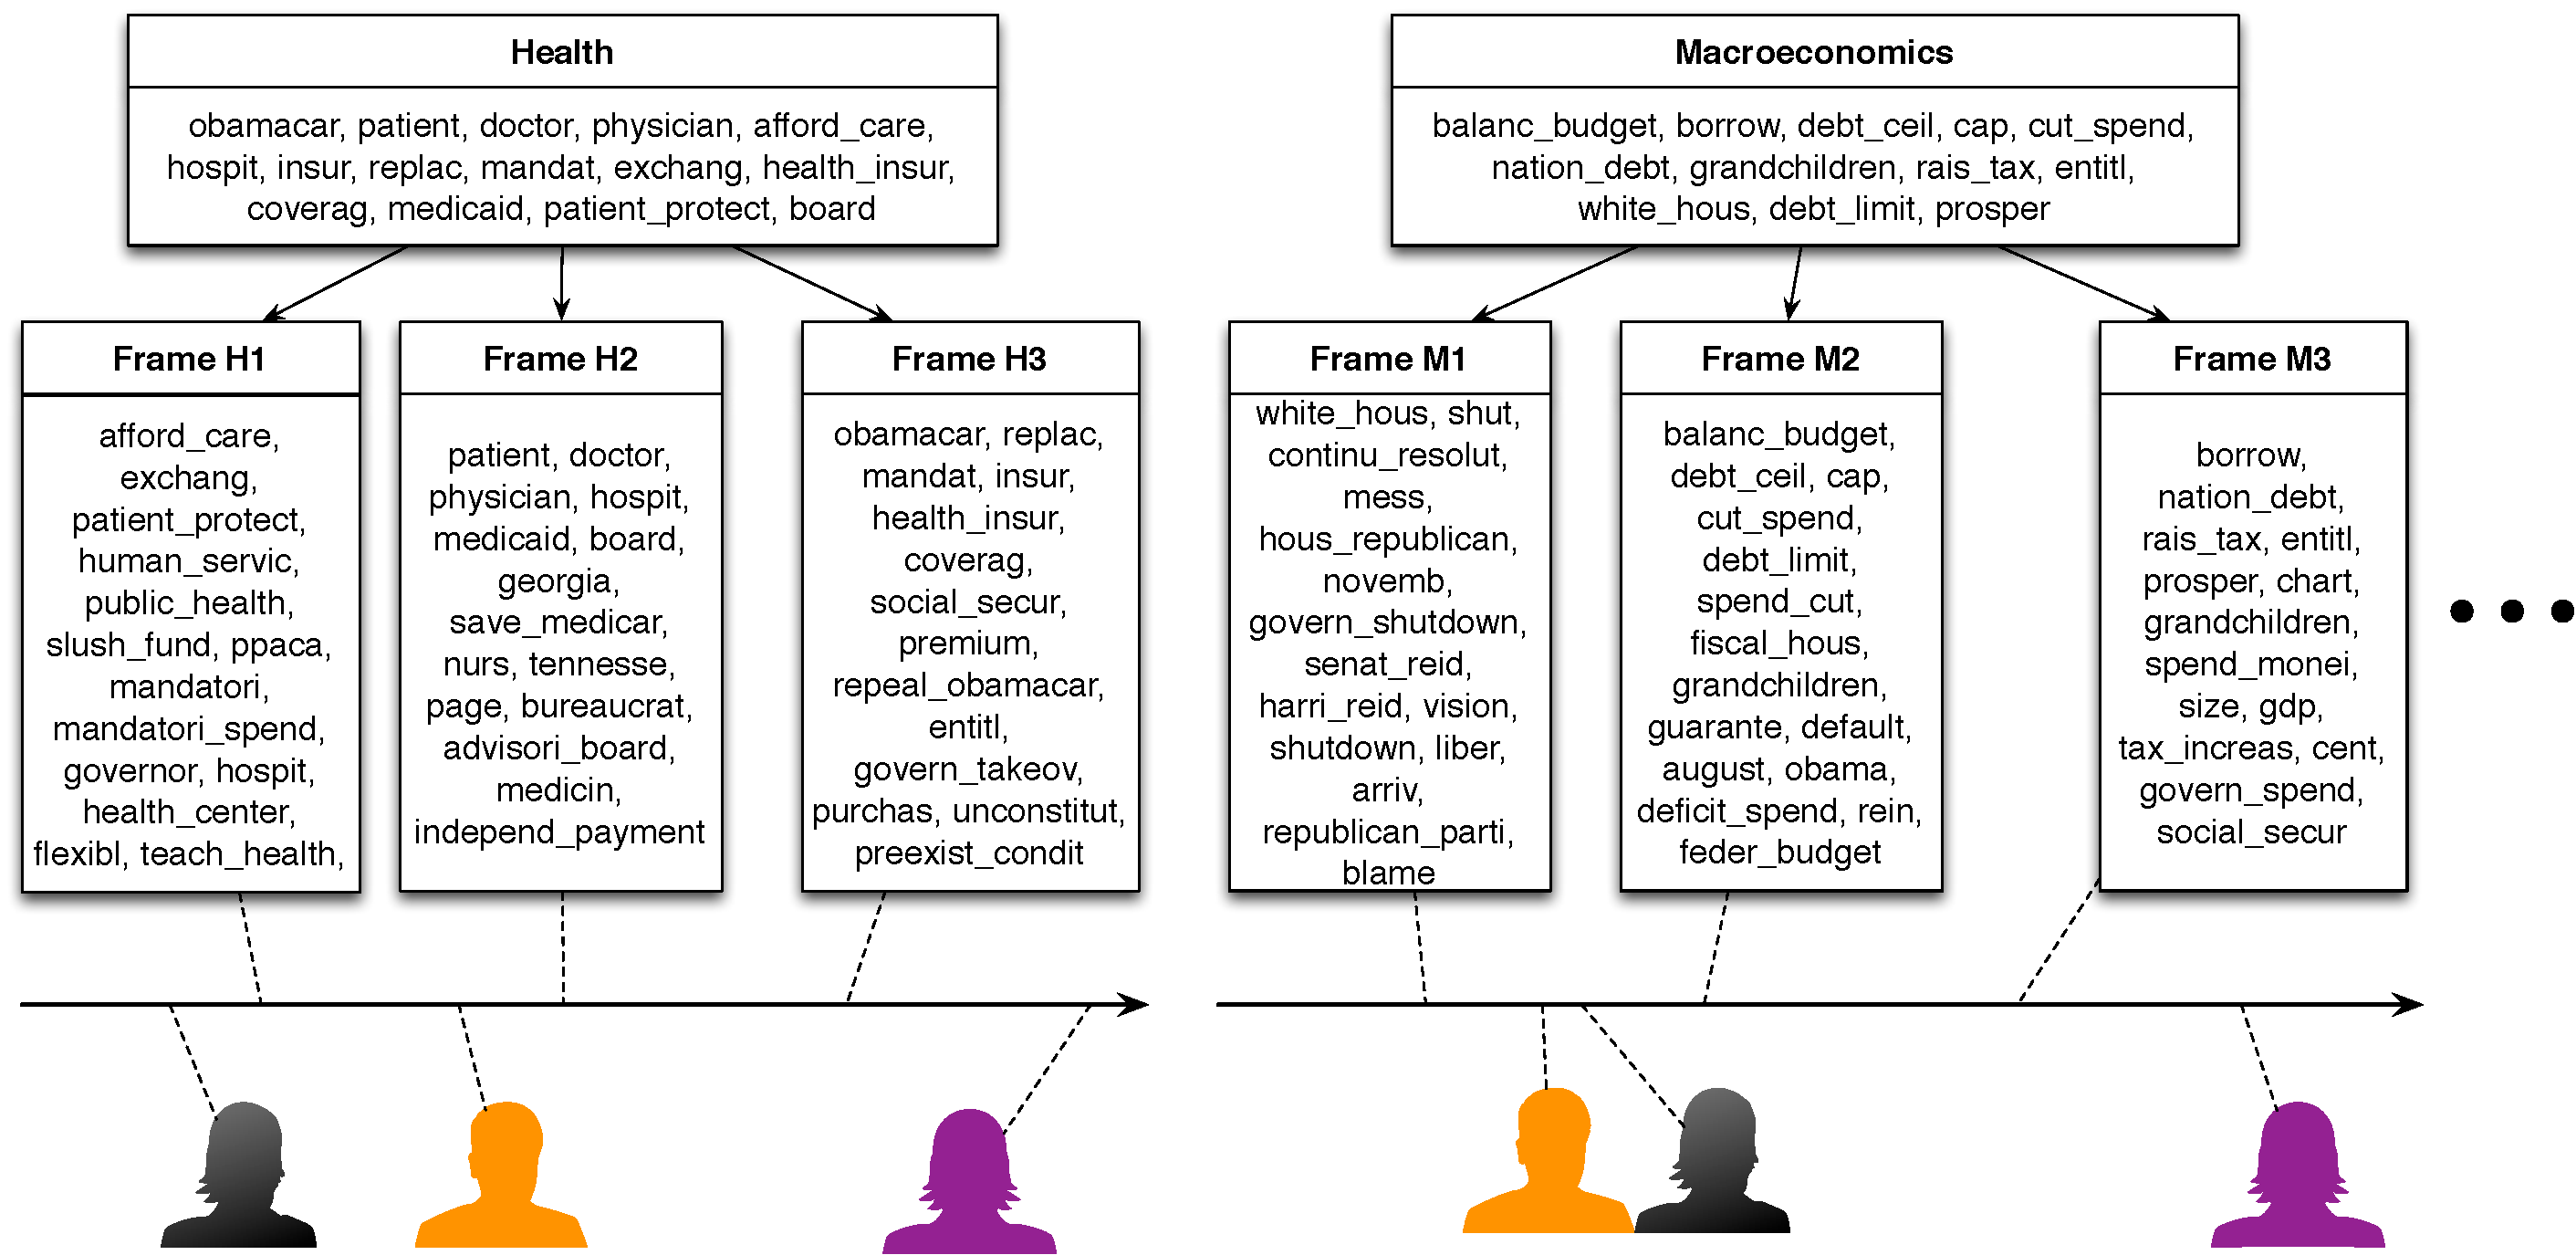
\includegraphics[width=\textwidth]{teaparty/figures/s5/expected_output}
    \end{figure}
}

\frame{
    \frametitle{Hierarchical Ideal Point Topic Model: Overview}
    \only<1-5>{
    \begin{block}{Using both votes and text to learn}
        \begin{itemize}
          \item Two-level topic hierarchy:
            \only<2>{
            \begin{itemize} 
            \item \alert<2>{First-level nodes map to agenda issues}
            \item \alert<2>{Second-level nodes map to issue-specific frames}
	   \end{itemize}}
            \only<3>{\alert<3>{Use existing labeled data to learn priors for interpretable
                issues}}
            \only<4>{ \alert<4>{Ideal points for frames for predictions using text only}}

          \item\alert<5>{Ideal points in multiple interpretable dimensions}
        \end{itemize}
    \end{block}
    \vspace{-.5cm}
    \begin{figure}
      \centering
      \only<1>{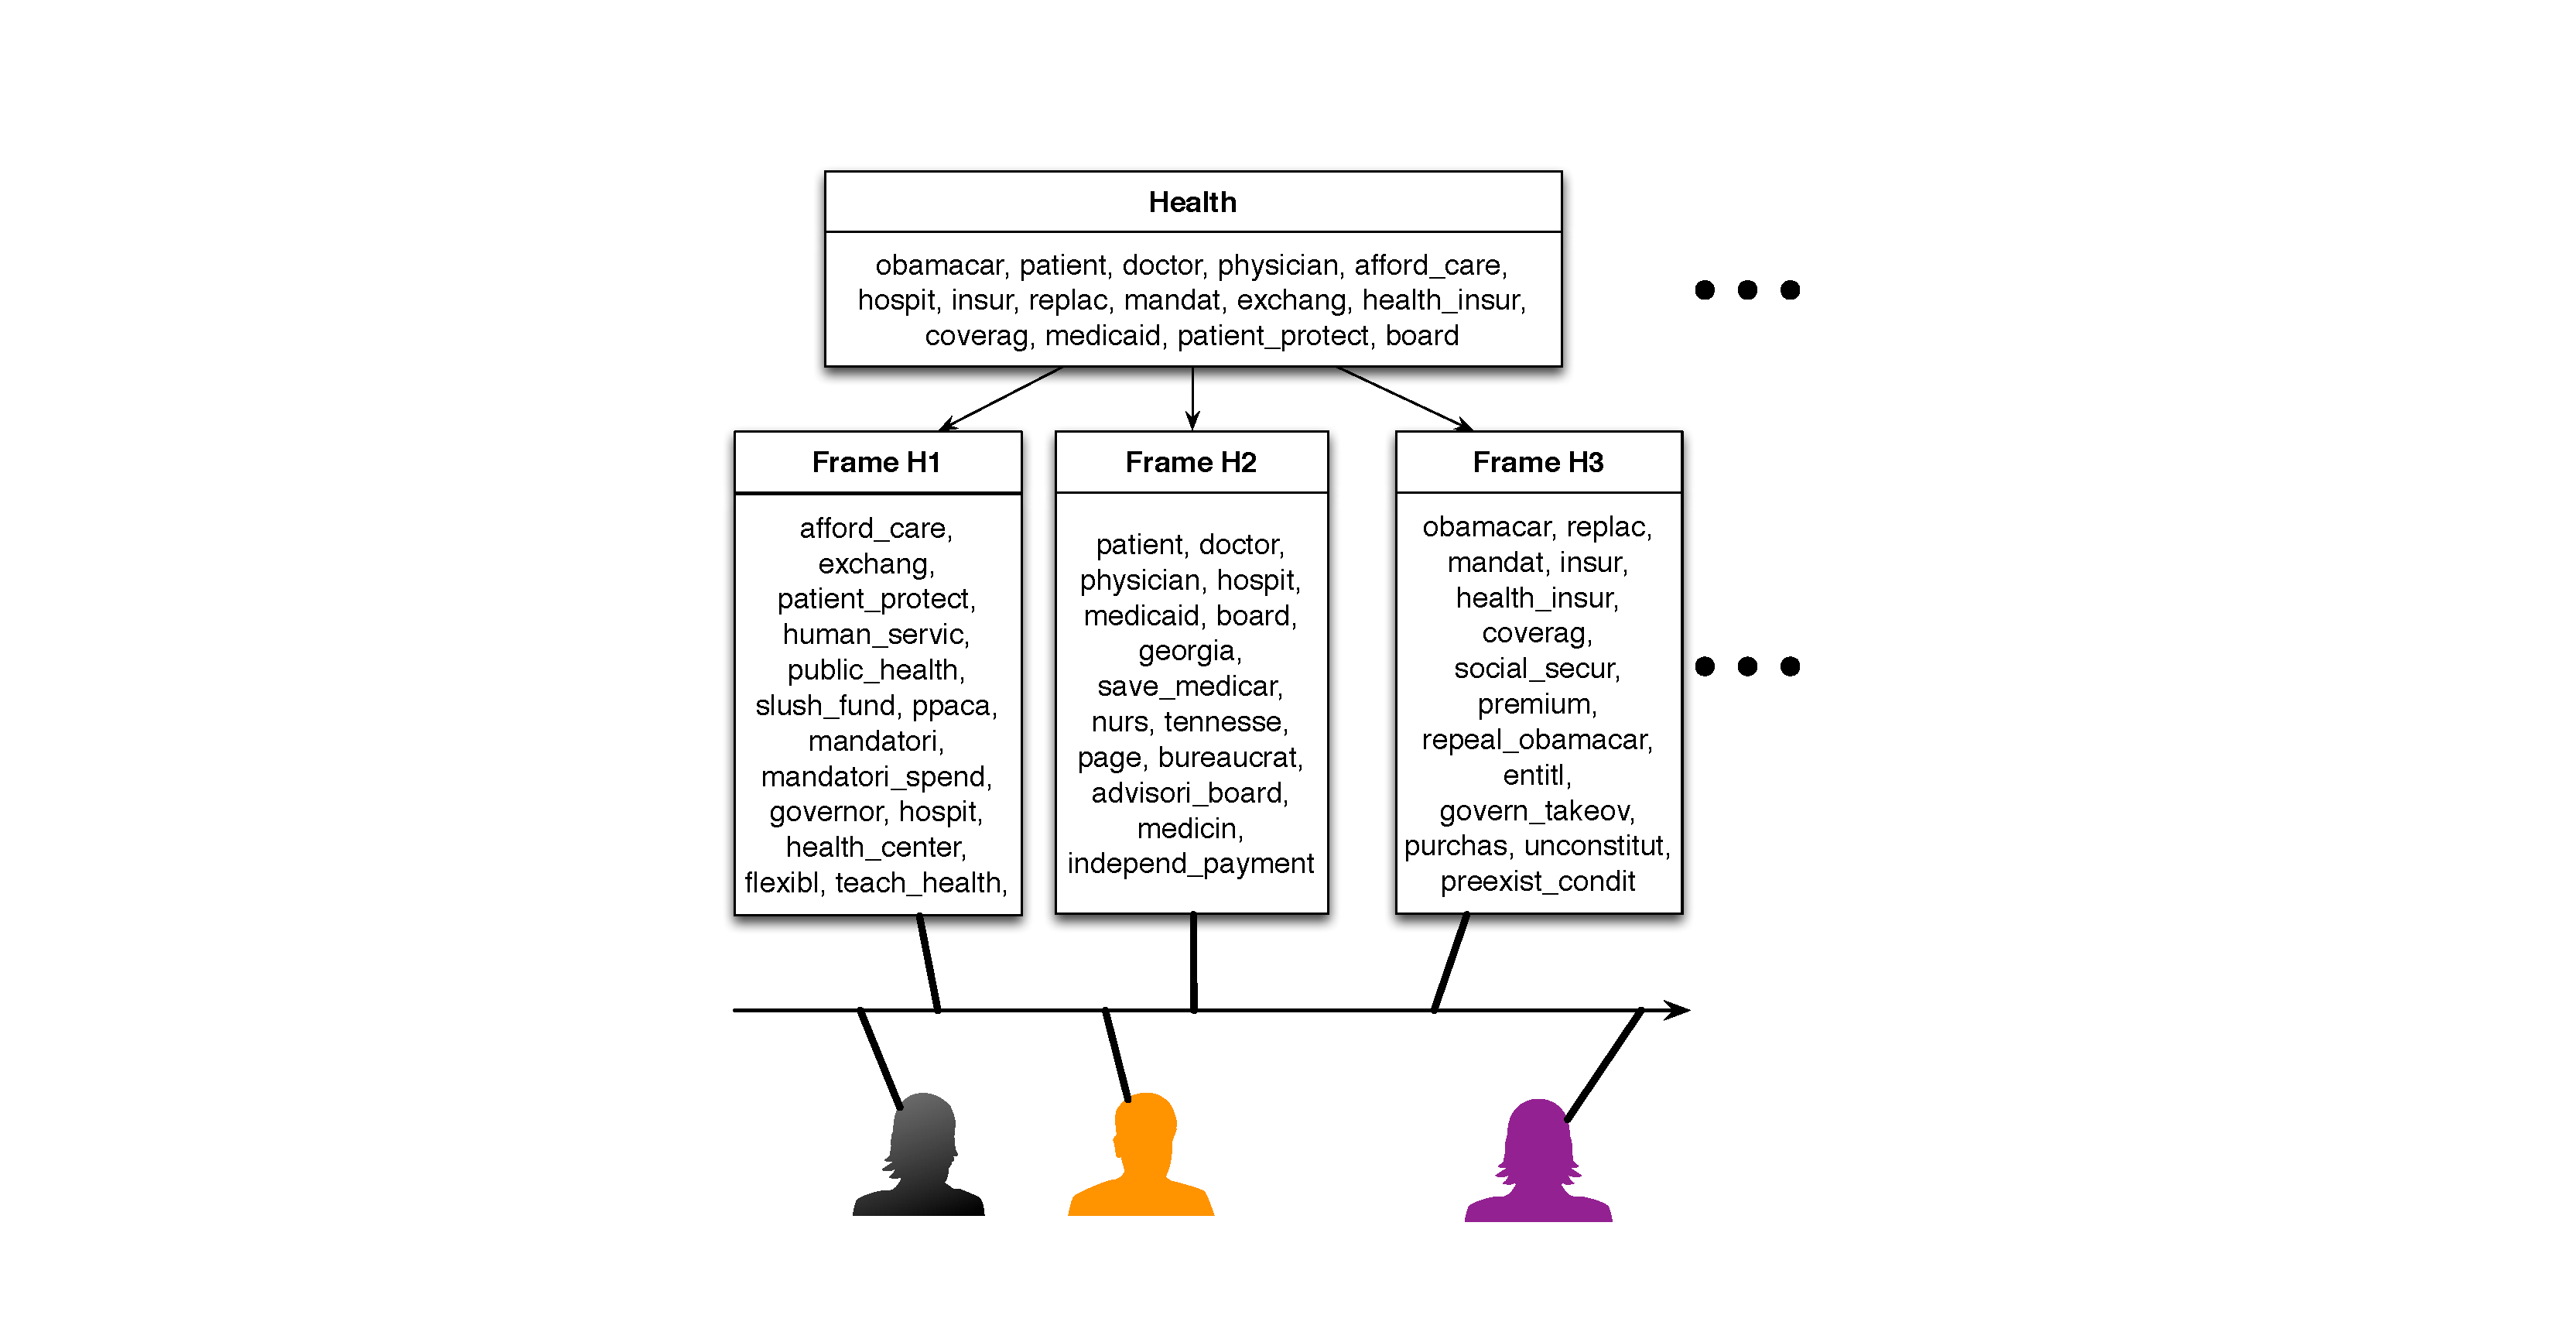
\includegraphics[width=.9\textwidth]{teaparty/figures/s5/output_1}}%
      \only<2>{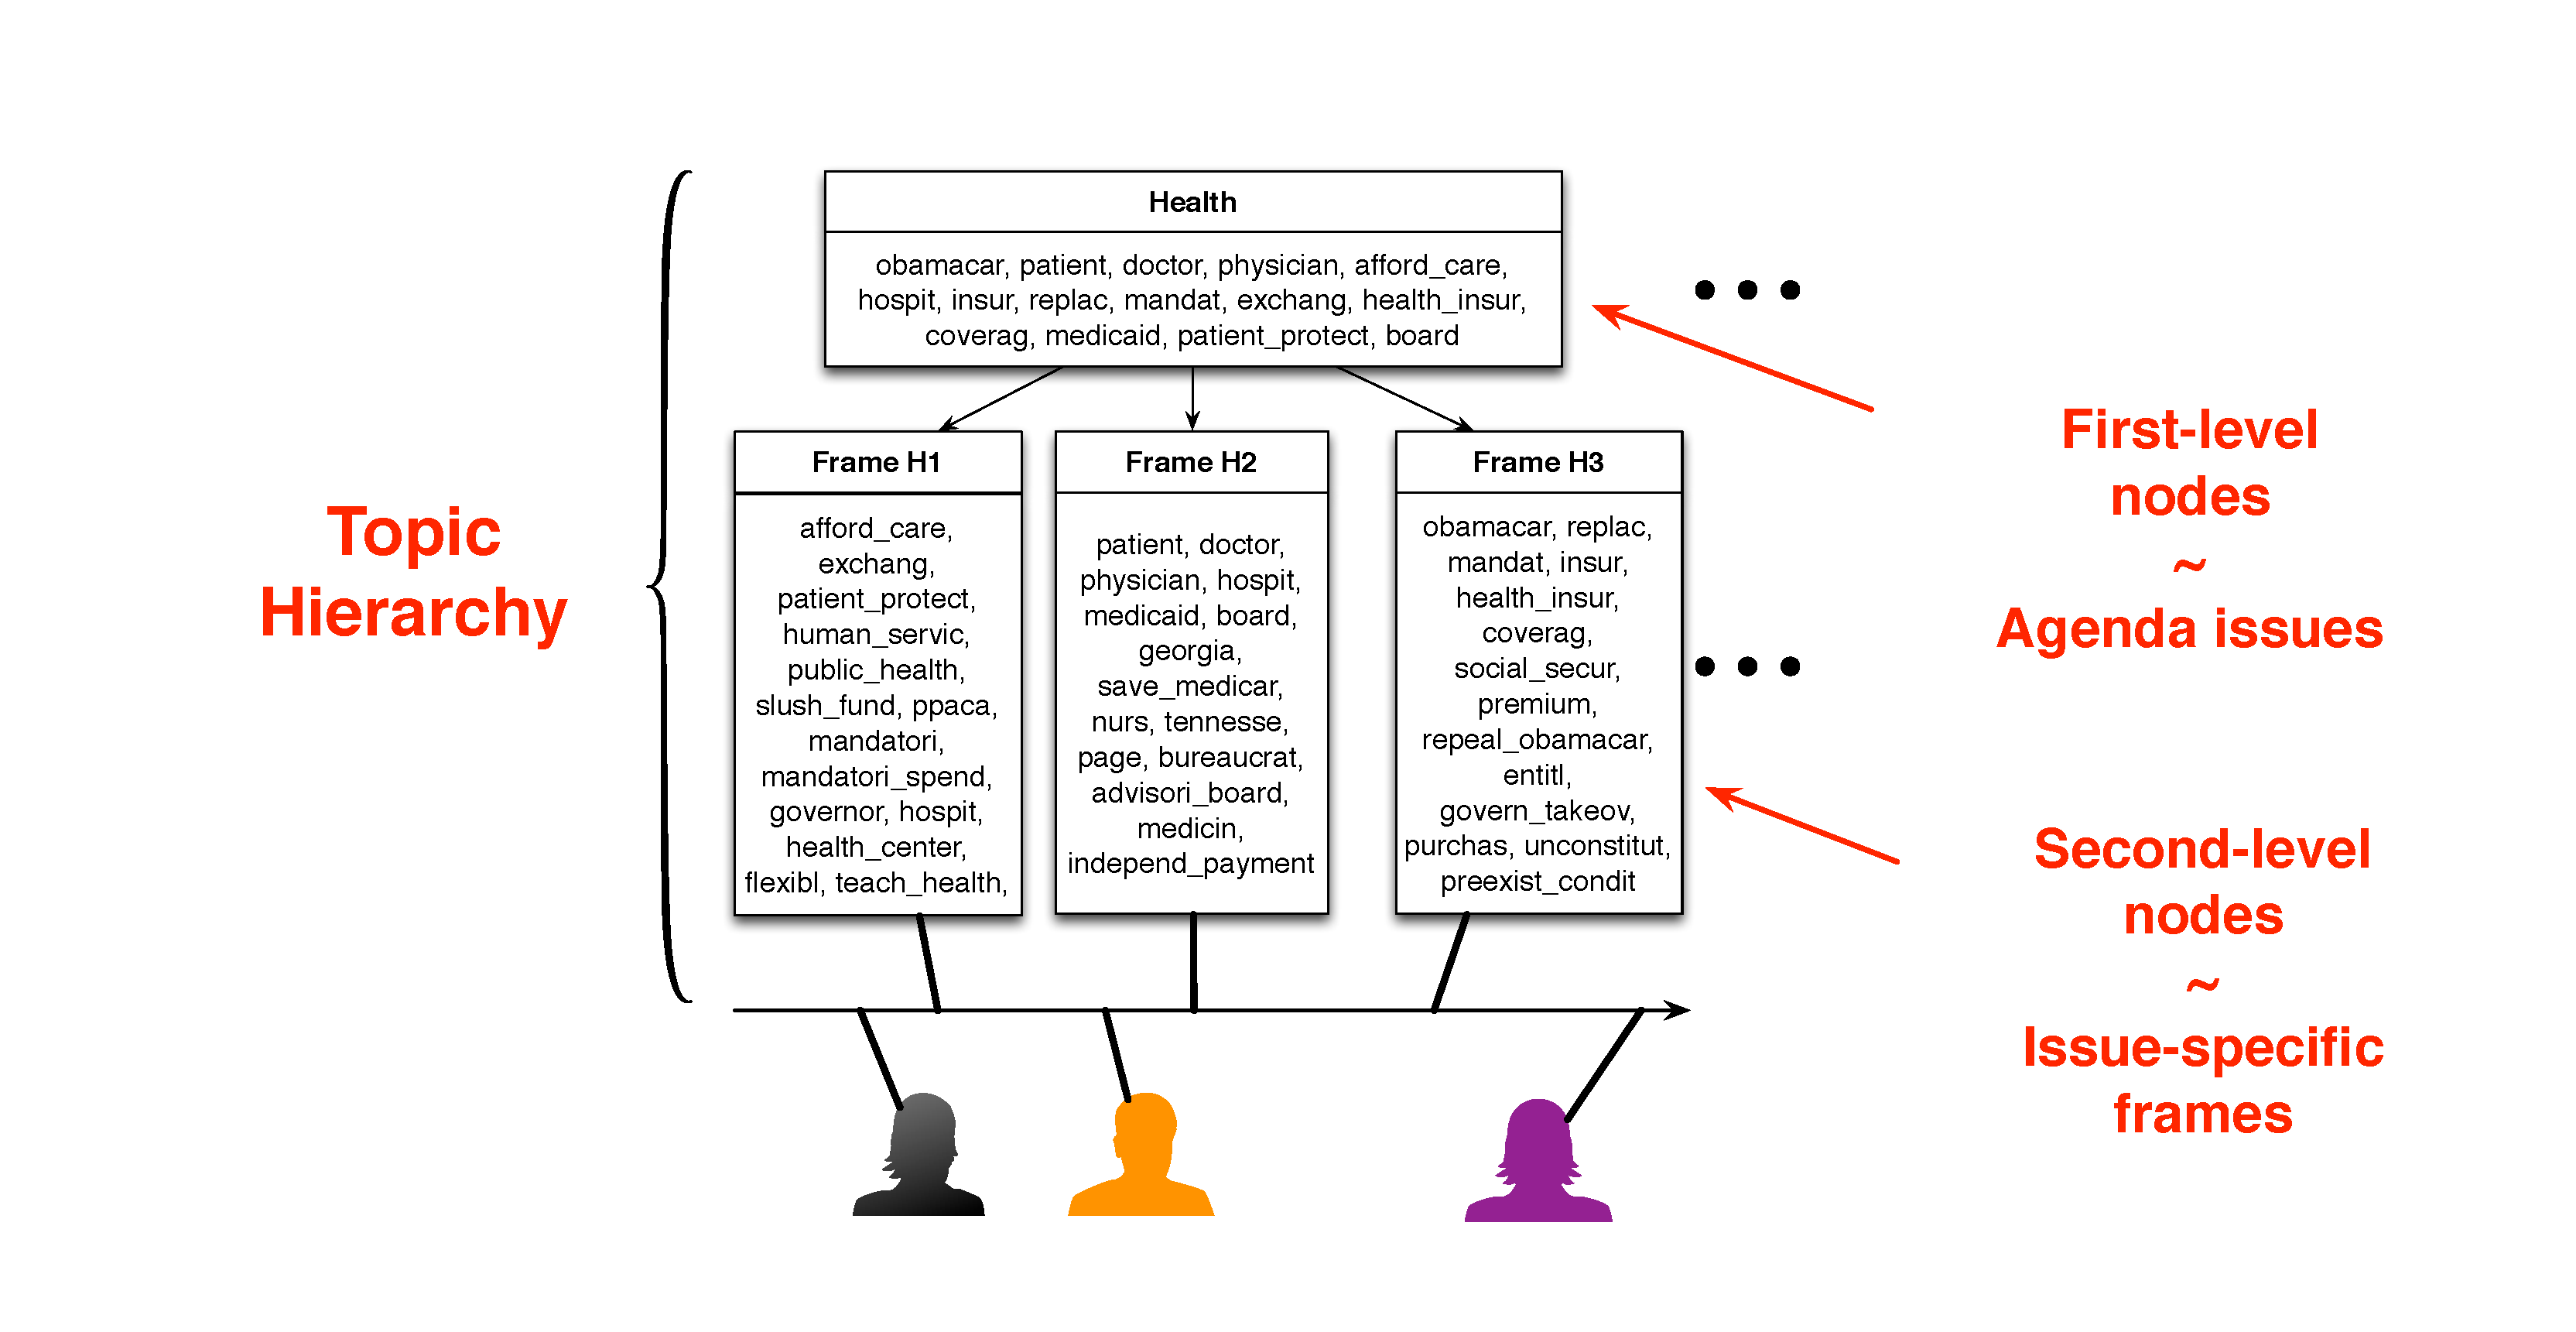
\includegraphics[width=.8\textwidth]{teaparty/figures/s5/output_2}}%
      \only<3>{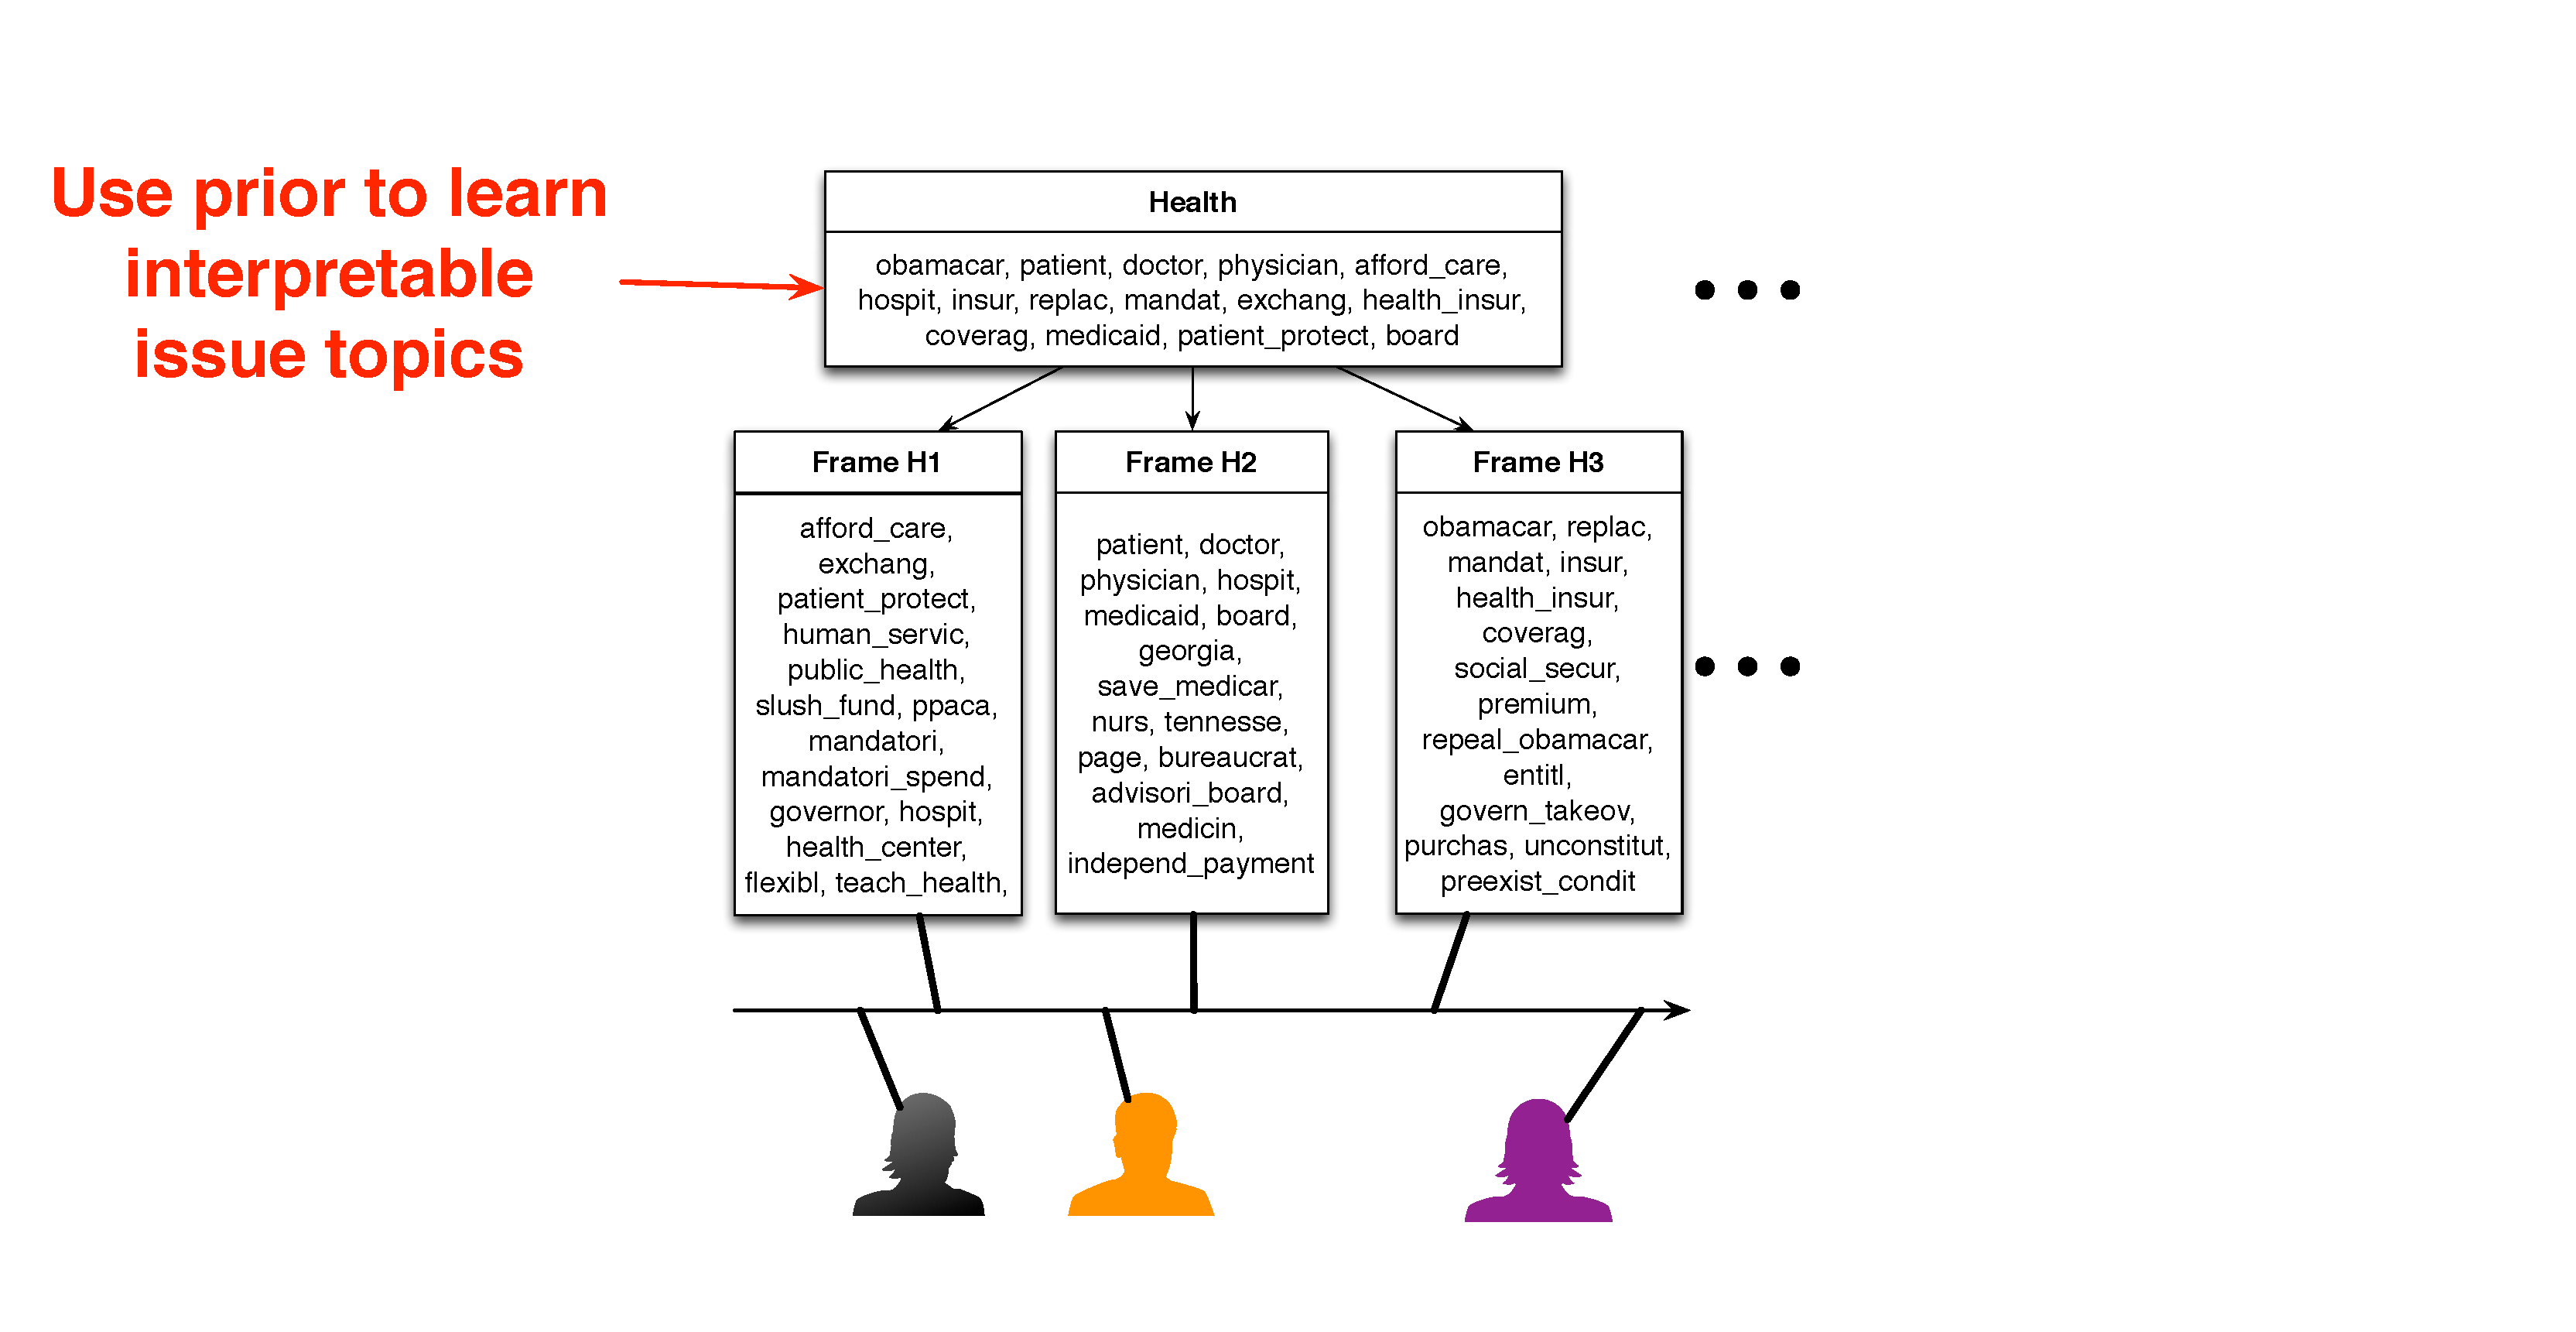
\includegraphics[width=.9\textwidth]{teaparty/figures/s5/output_4}}%
      \only<4>{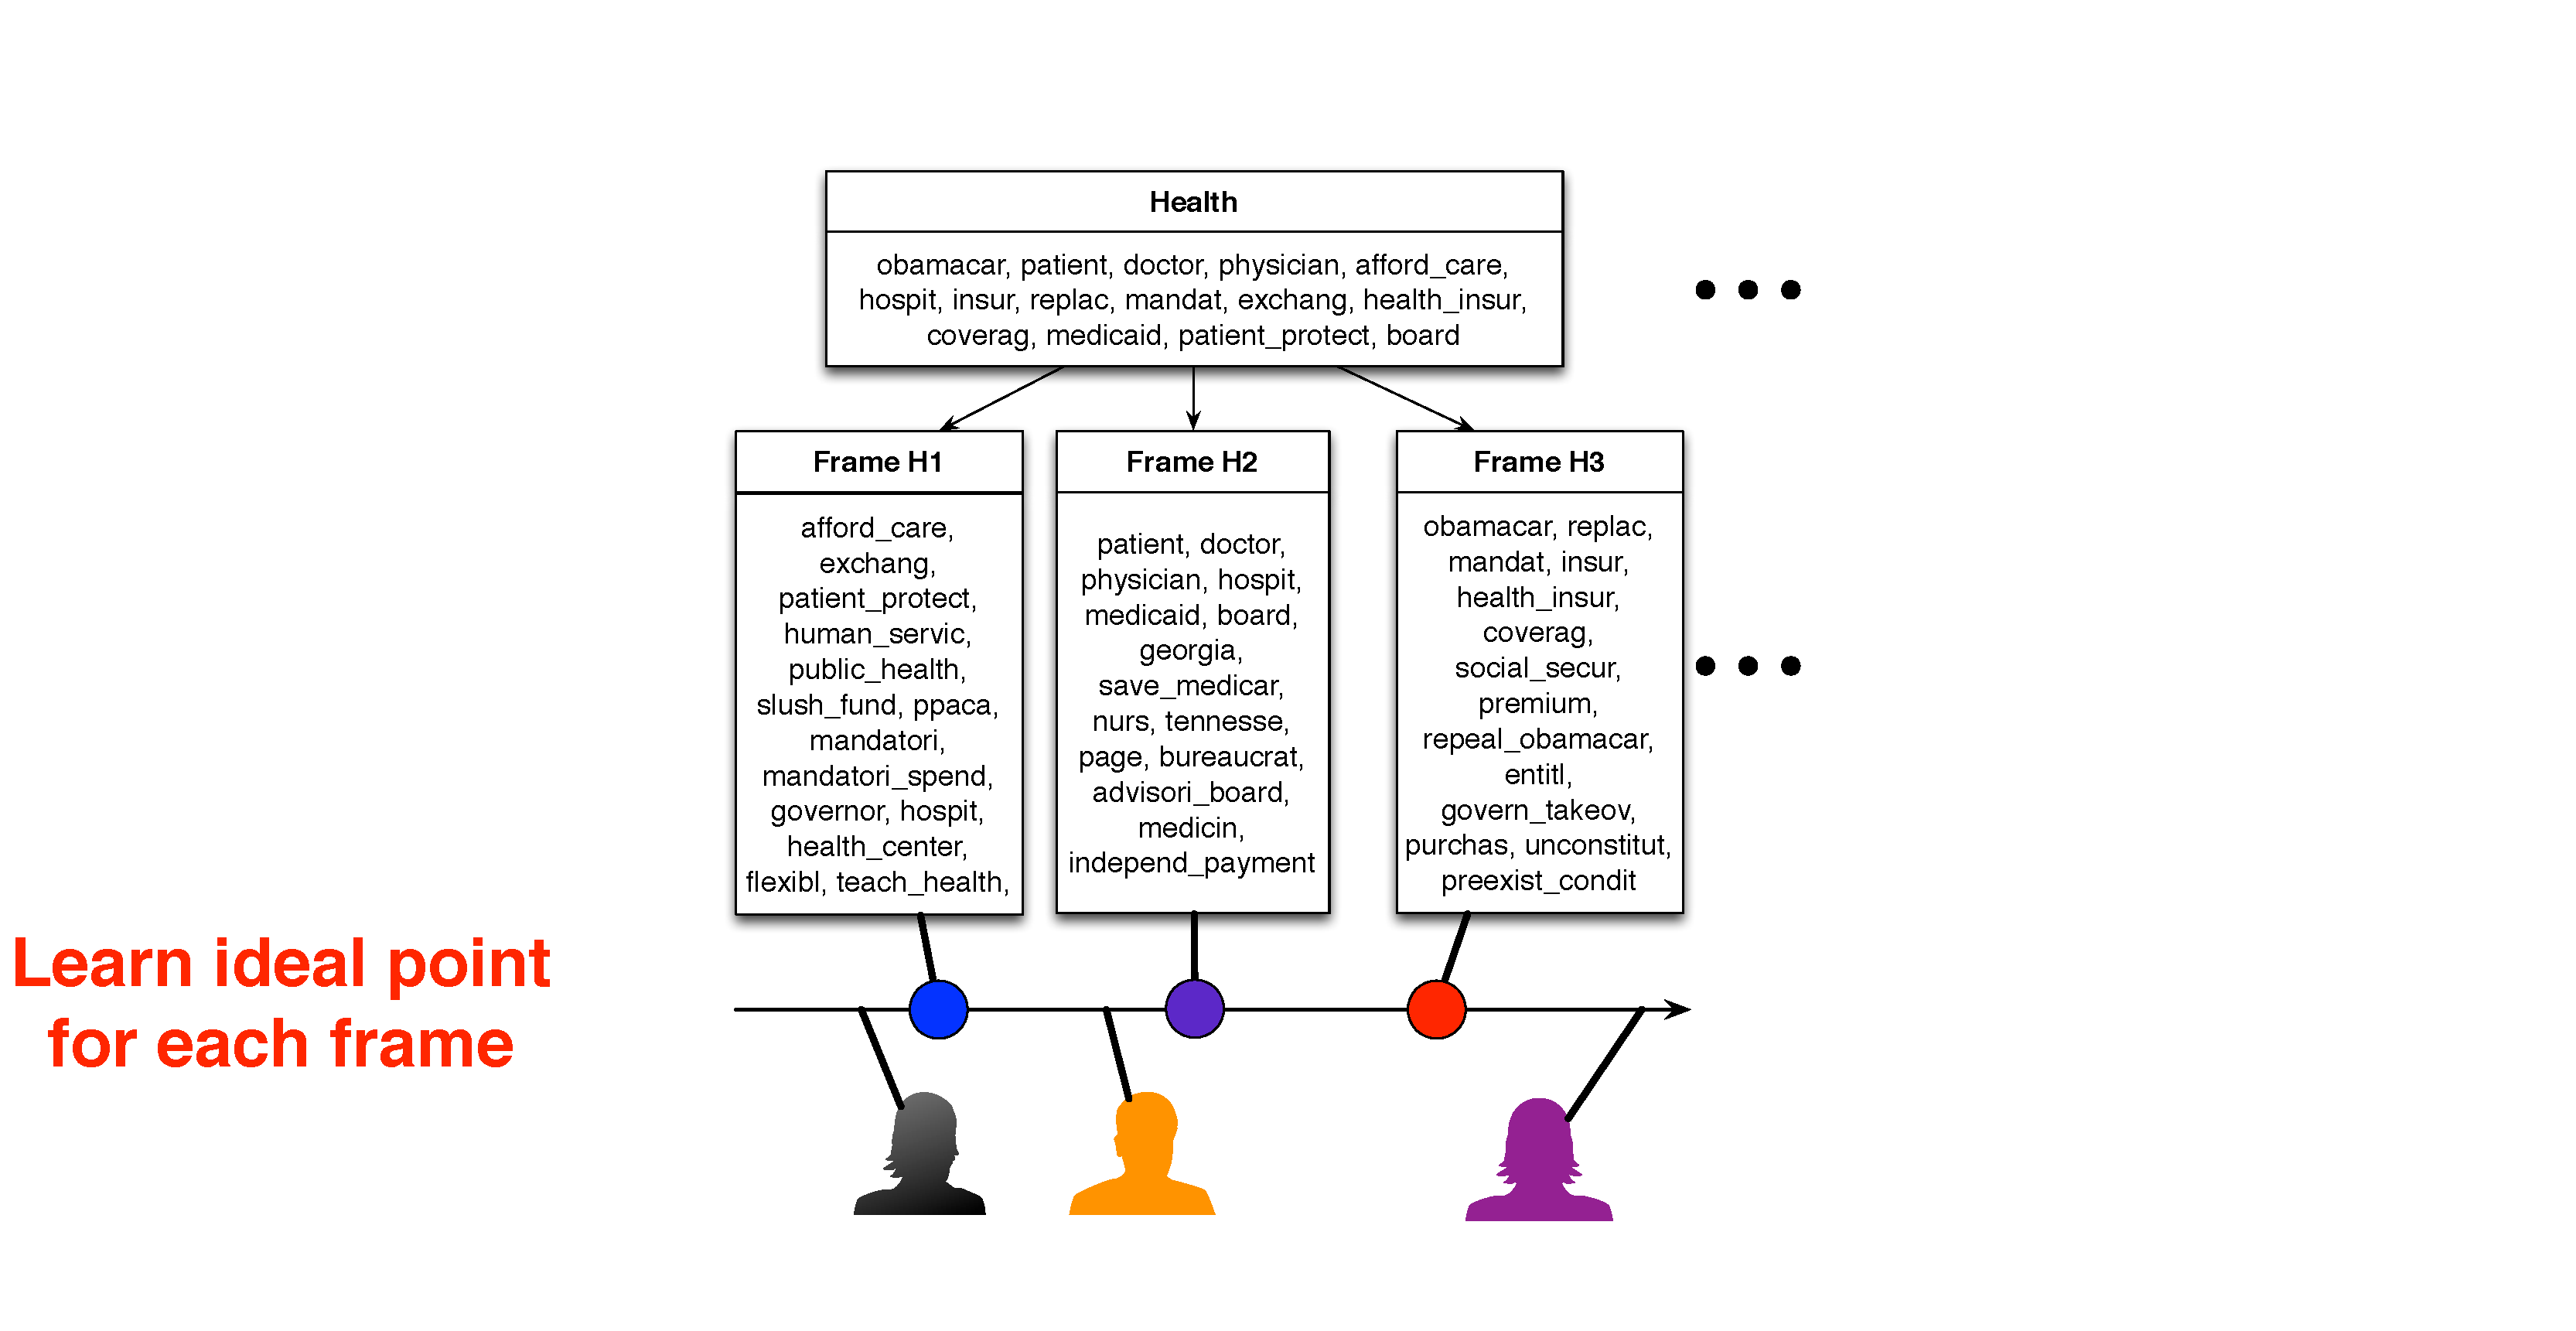
\includegraphics[width=.9\textwidth]{teaparty/figures/s5/output_5}}%
      \only<5>{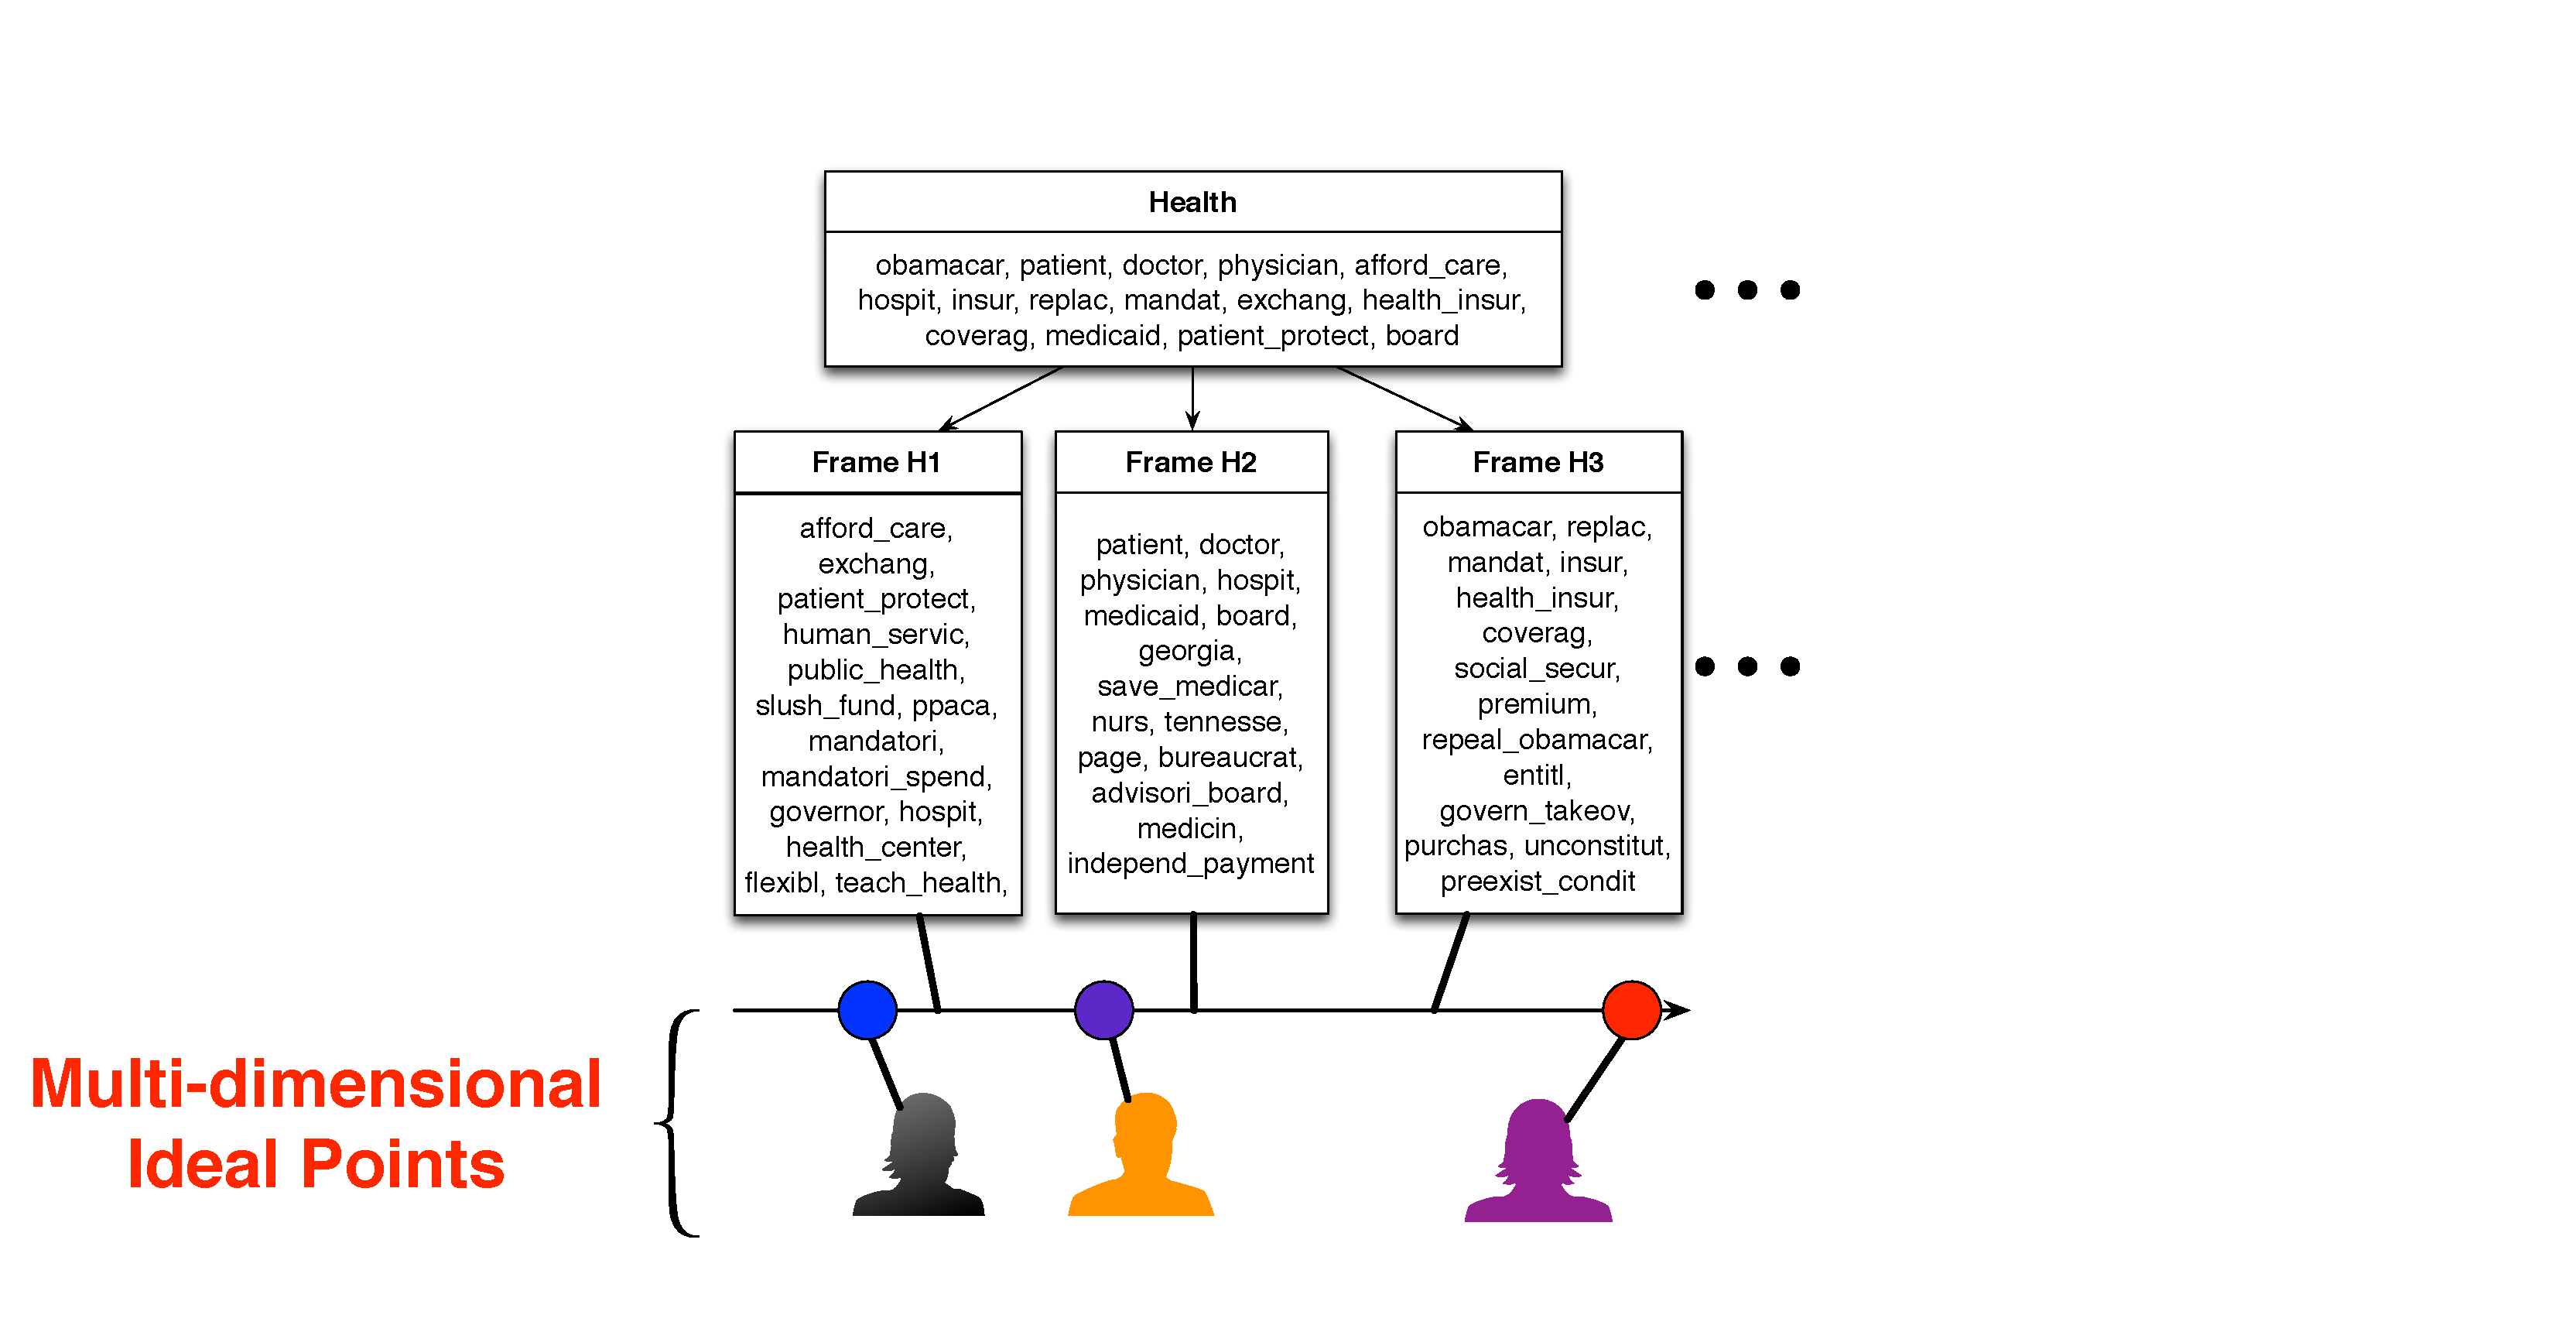
\includegraphics[width=.9\textwidth]{teaparty/figures/s5/output_3}}%
    \end{figure}
    }

    \only<6>{
    \begin{block}{Hierarchical Ideal Point Topic Model: Inputs}
      \begin{itemize}
        \item A collection of votes $\{v \subtwo ab\}$
        \item A collection of $D$ speeches $\{\bm w_d\}$, each of which is given by legislator
            $a_d$
        \item A collection of $B$ bill text $\{\bm w'_b\}$
      \end{itemize}
    \end{block}
    \begin{center}
      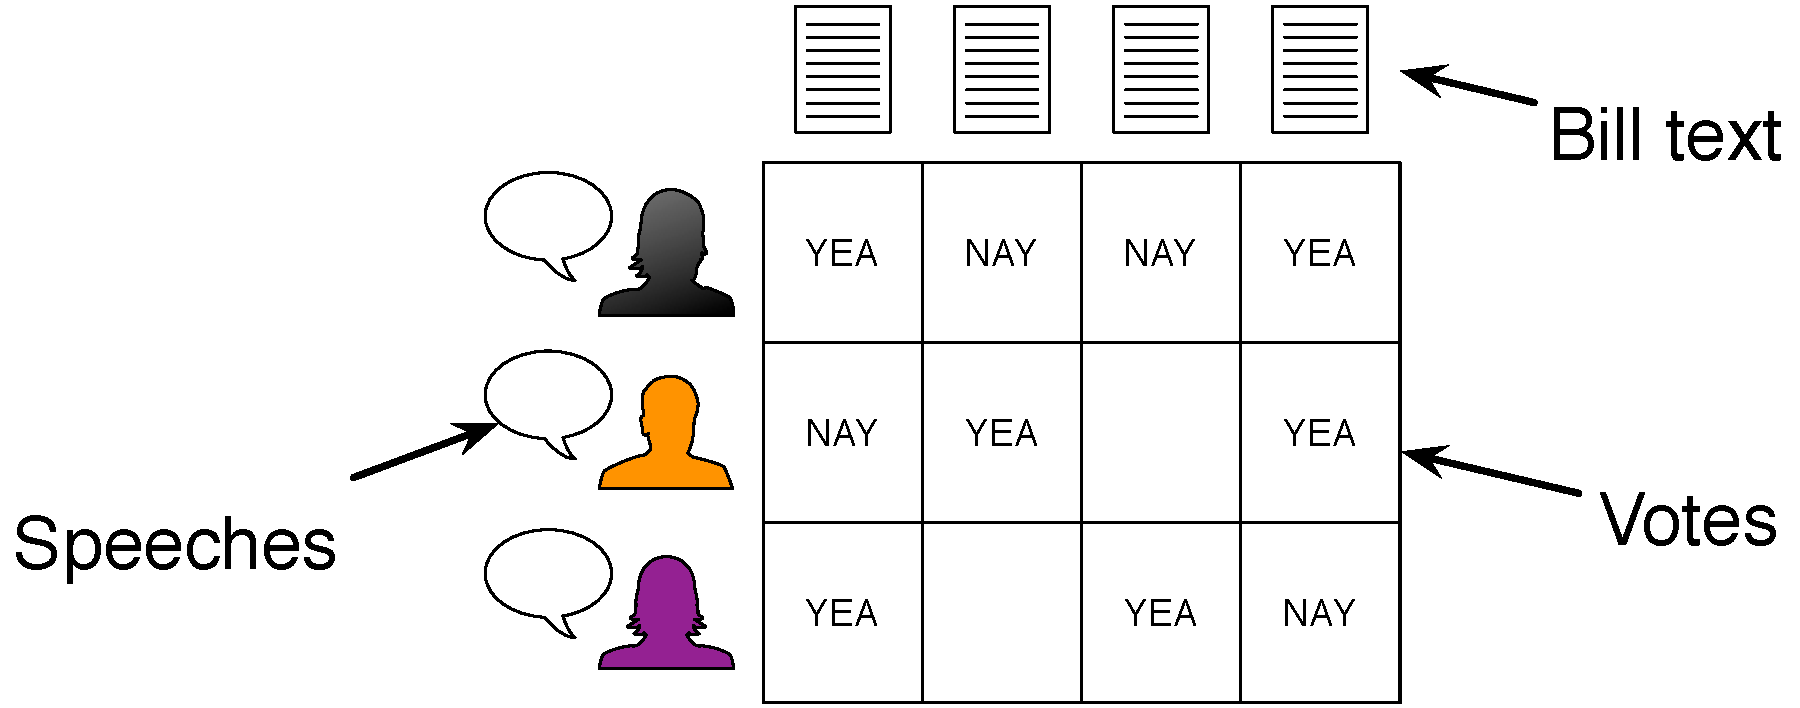
\includegraphics[width=.75\textwidth]{teaparty/figures/s5/data}%
    \end{center}
    }
}

\frame{
    \frametitle{Hierarchical Ideal Point Topic Model}
    \only<1>{
    \begin{overlayarea}{\linewidth}{3.5cm}
    \begin{block}{Modeling bill text}
        \begin{itemize}
          \item Each bill text $b$ is a mixture over $K$ issues $\vartheta_b$
          \item Each bill token generated from topic at \redtext{first-level issue node}
        \end{itemize}
    \end{block}
    \end{overlayarea}
    \vspace{-1.2cm}
    \begin{center}
      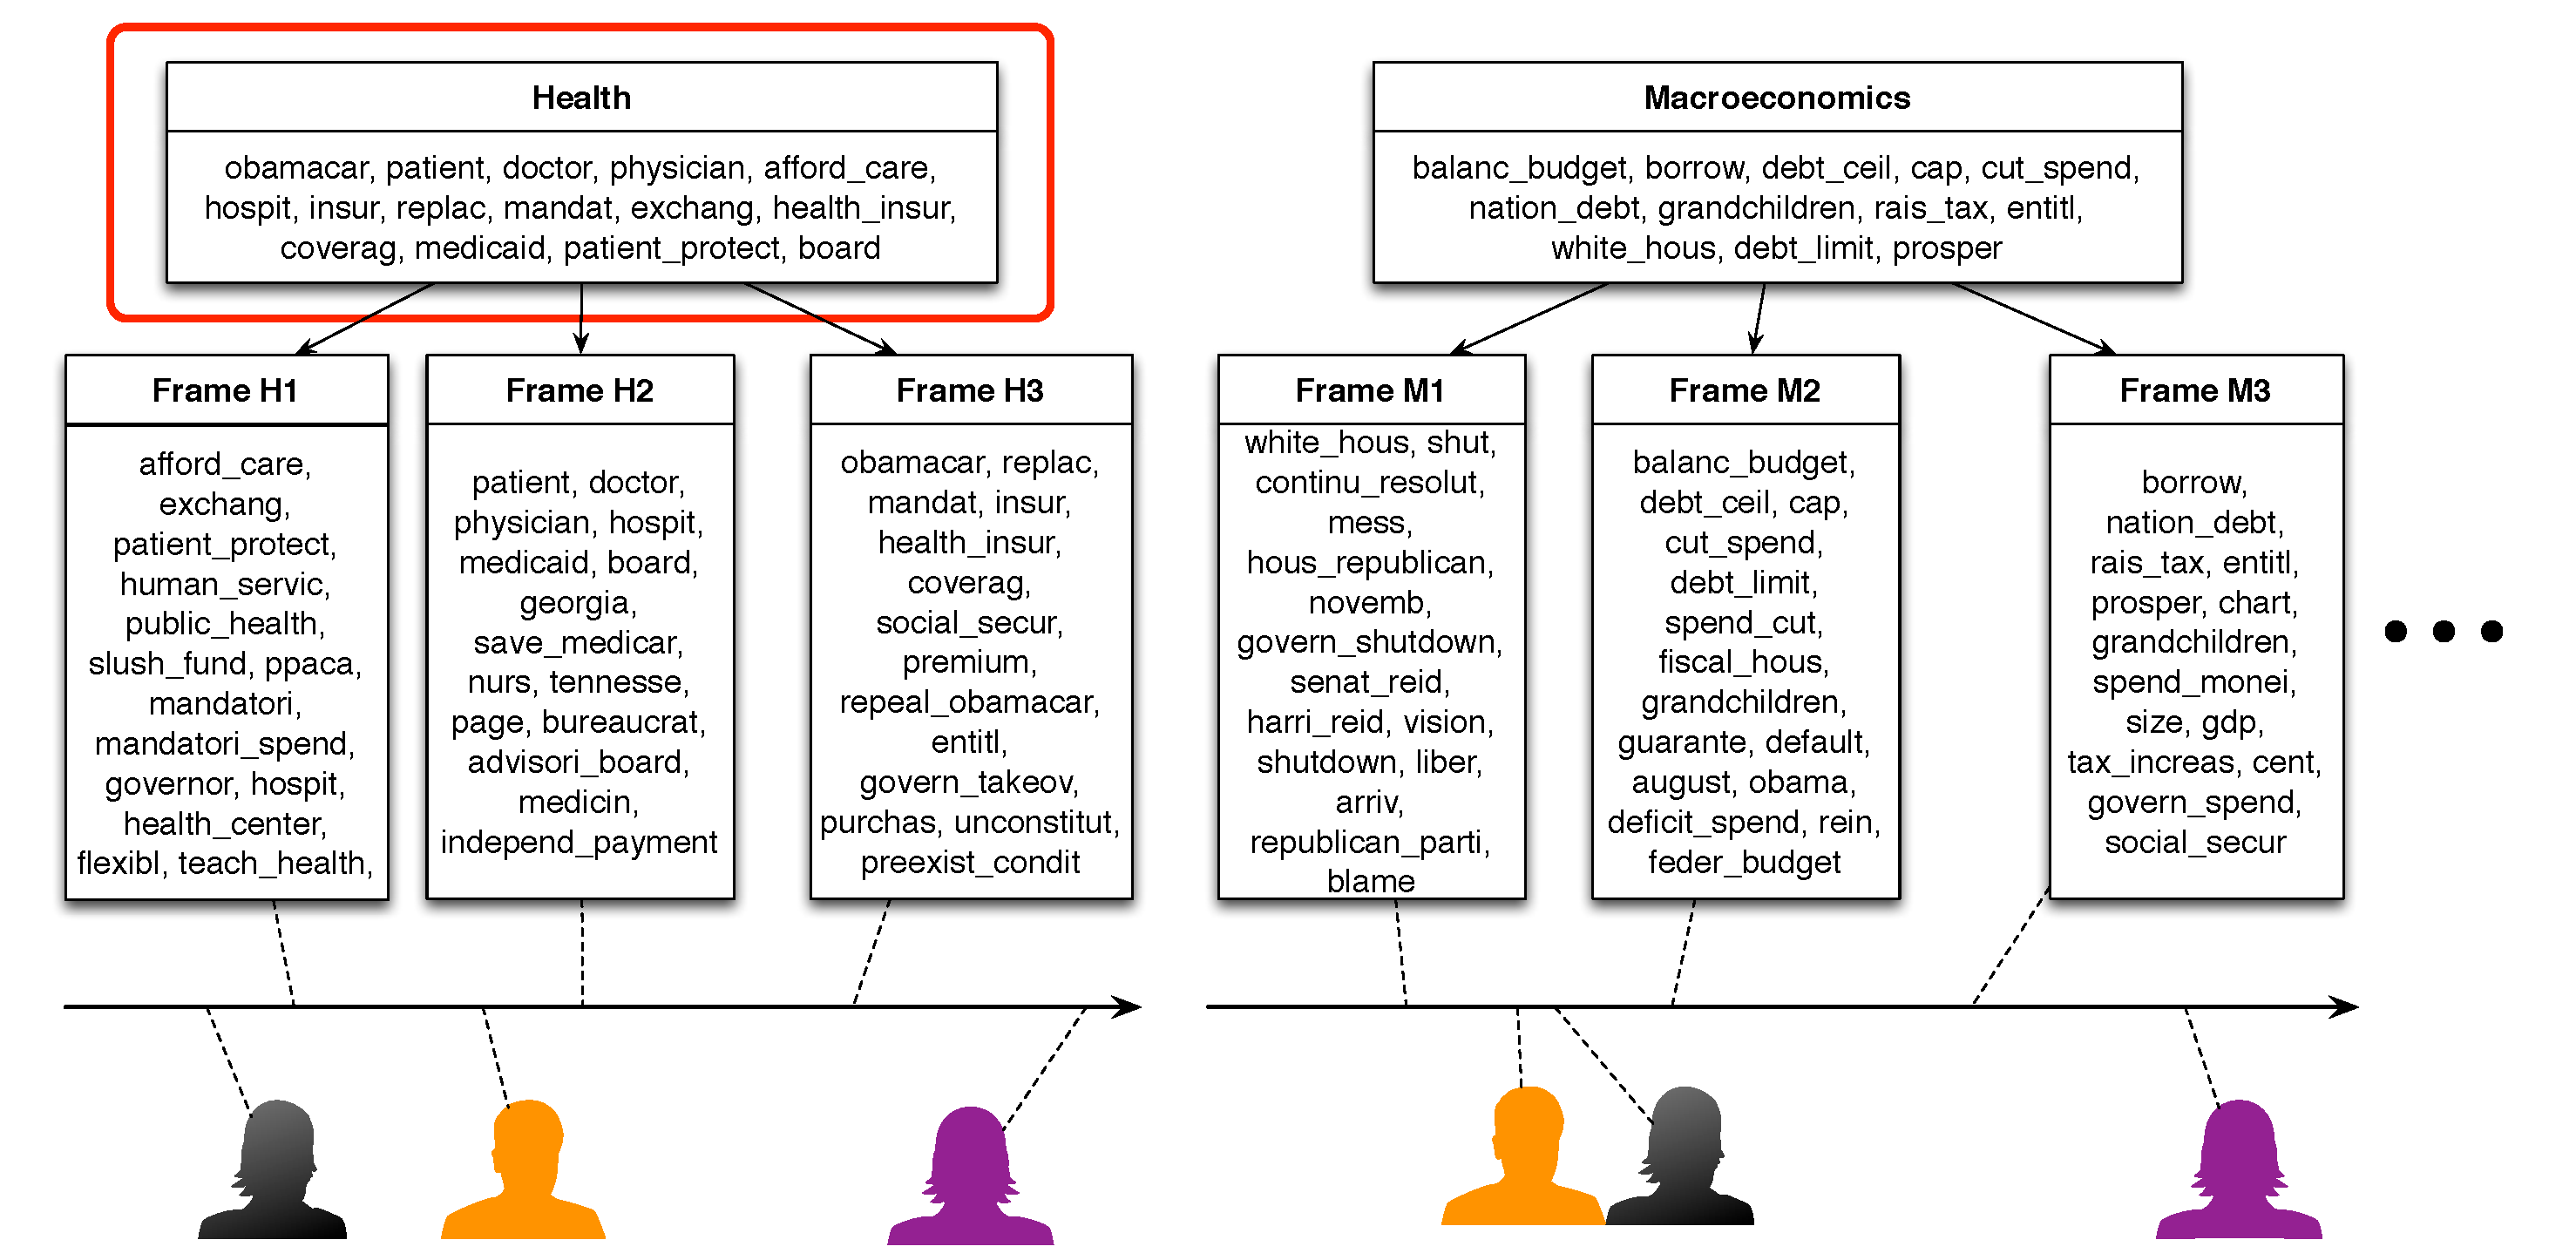
\includegraphics[width=.8\textwidth]{teaparty/figures/s5/modeling_bills}
    \end{center}
    }

    \only<2>{
    \begin{overlayarea}{\linewidth}{3.5cm}
    \begin{block}{Hierarchical Ideal Point Topic Model: Generative Process}
        \begin{itemize}
          \item Each speech $d$ also has a distribution $\theta_d$ over $K$ issues
          \item Each issue $k$, each speech $d$ has distribution over frames $\psi \subtwo dk$
          \item Each speech token from topic at \redtext{second-level frame
          node}
        \end{itemize}
    \end{block}
    \end{overlayarea}
    \vspace{-1cm}
    \begin{center}
      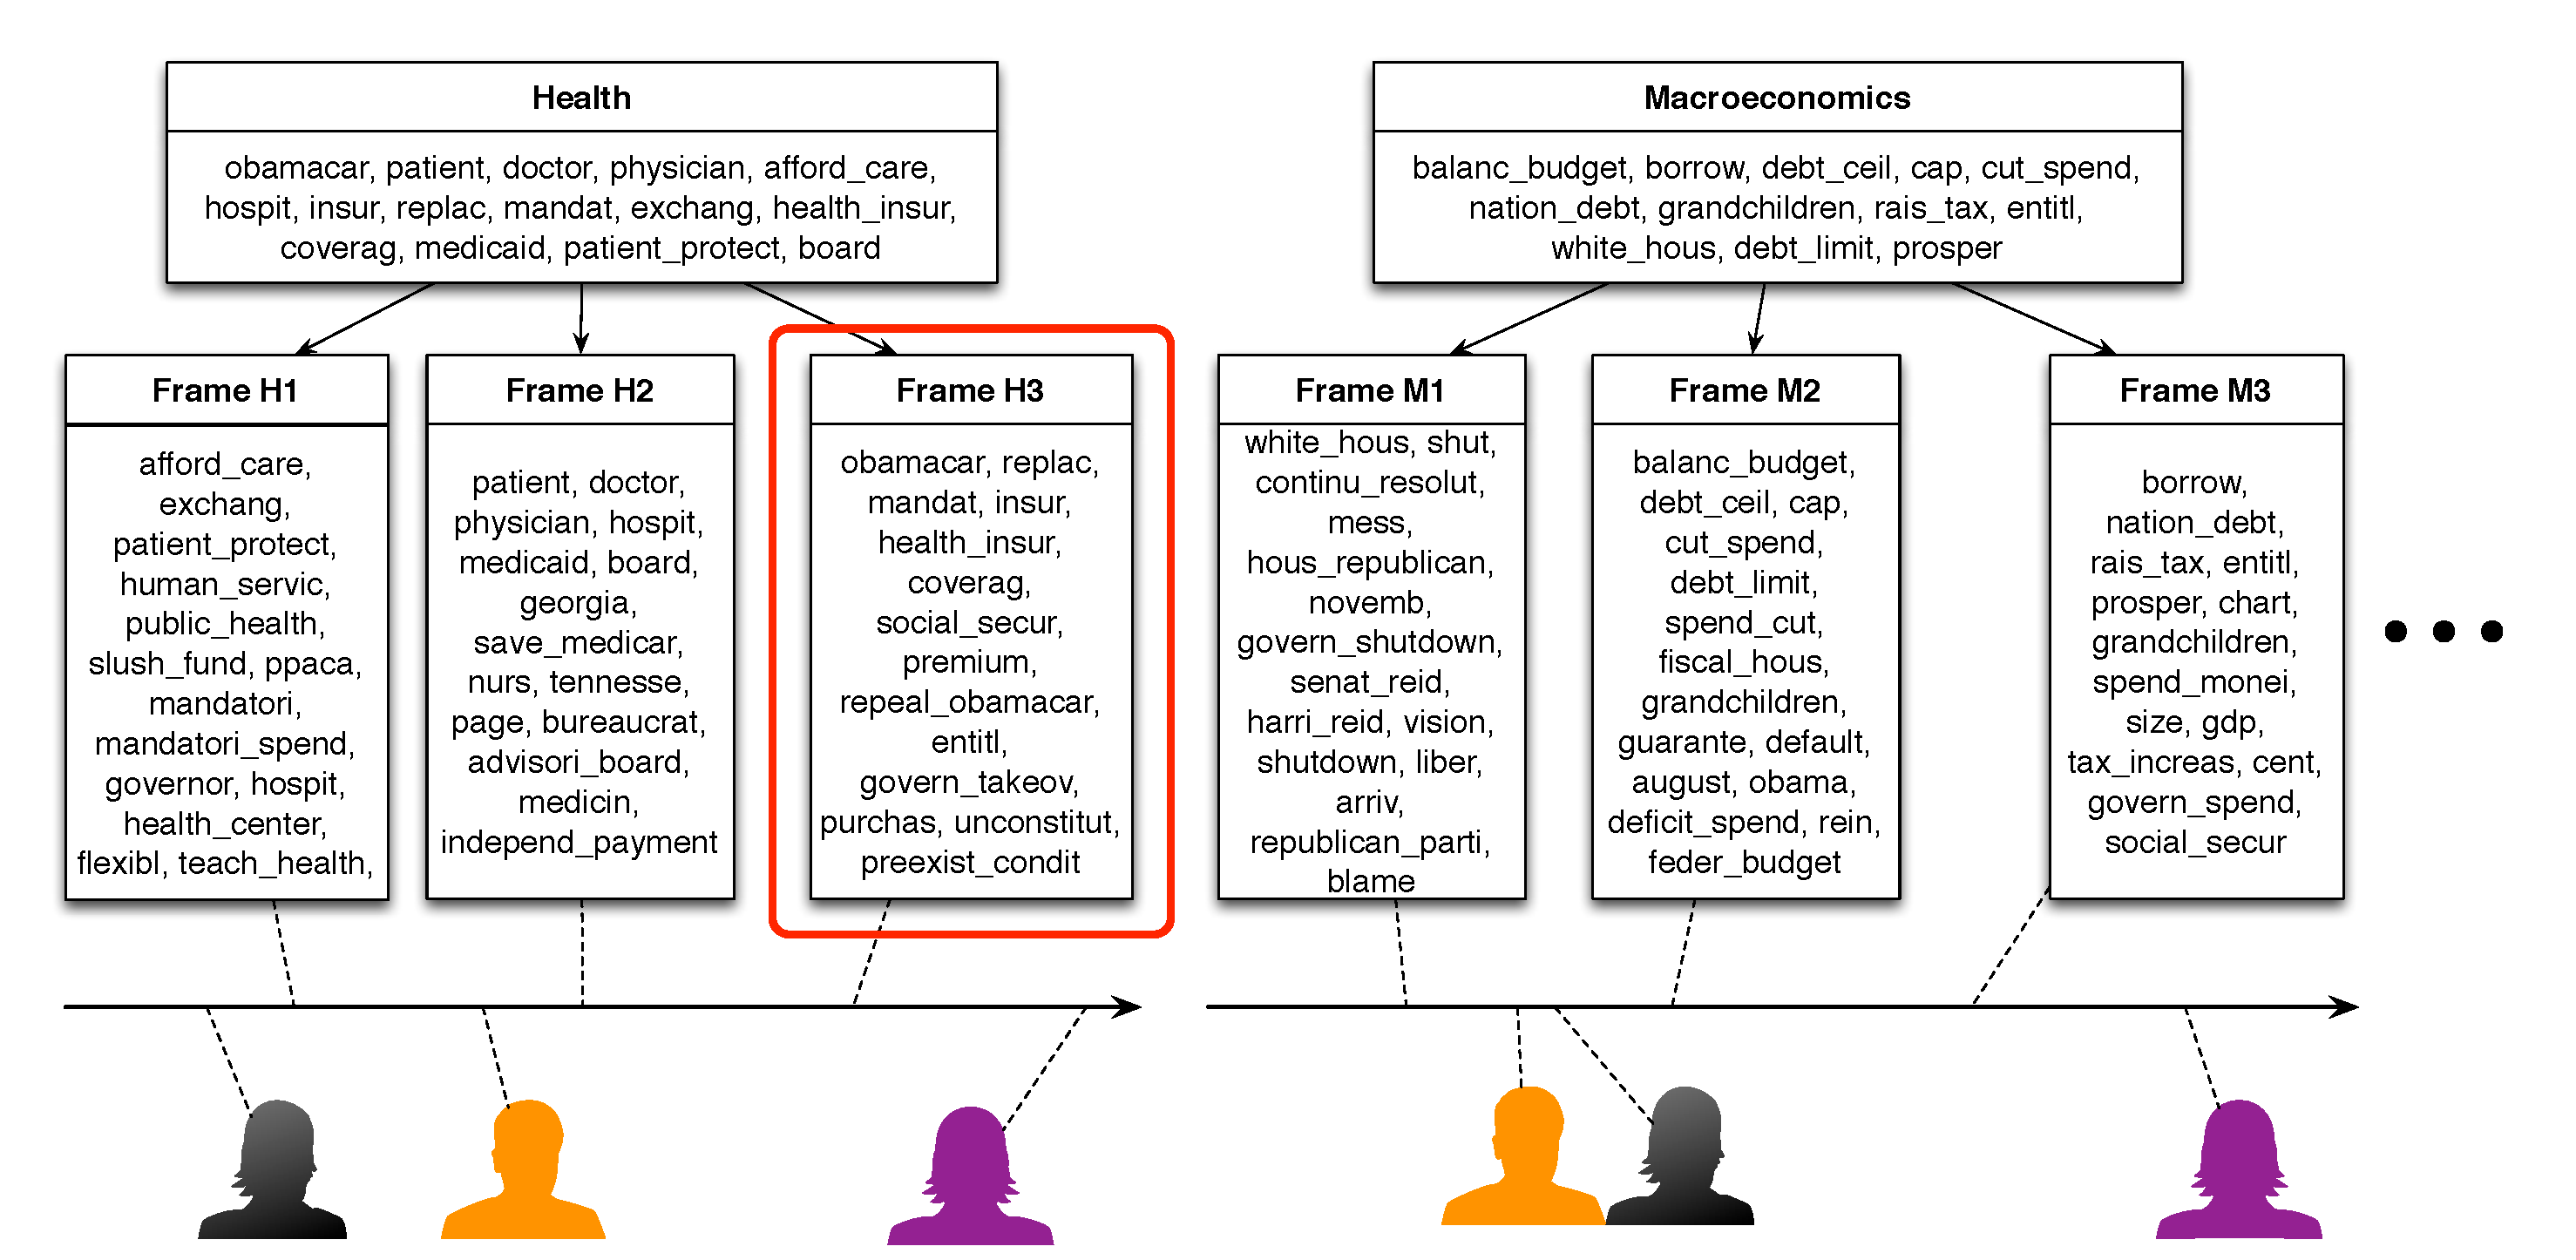
\includegraphics[width=.8\textwidth]{teaparty/figures/s5/modeling_speeches}
    \end{center}
    }

    \only<3>{
    \begin{overlayarea}{\linewidth}{3.5cm}
    \begin{block}{Hierarchical Ideal Point Topic Model: Modeling votes}
        \begin{itemize}
          \item Legislator $a$ votes `Yea' on bill $b$ with probability $p(v \subtwo ab = \mbox{Yea}) = \Phi(x_b \sum_{k=1}^K \vartheta \subtwo bk u \subtwo ak +
          y_b)$
          \item \redtext{Ideal point} $u \subtwo ak \sim \mathcal{N}(\sum_{j=1}^{J_k} \eta \subtwo kj \psi \subthree akj, \rho)$
        \end{itemize}
    \end{block}
    \end{overlayarea}
    \vspace{-1cm}
    \begin{center}
      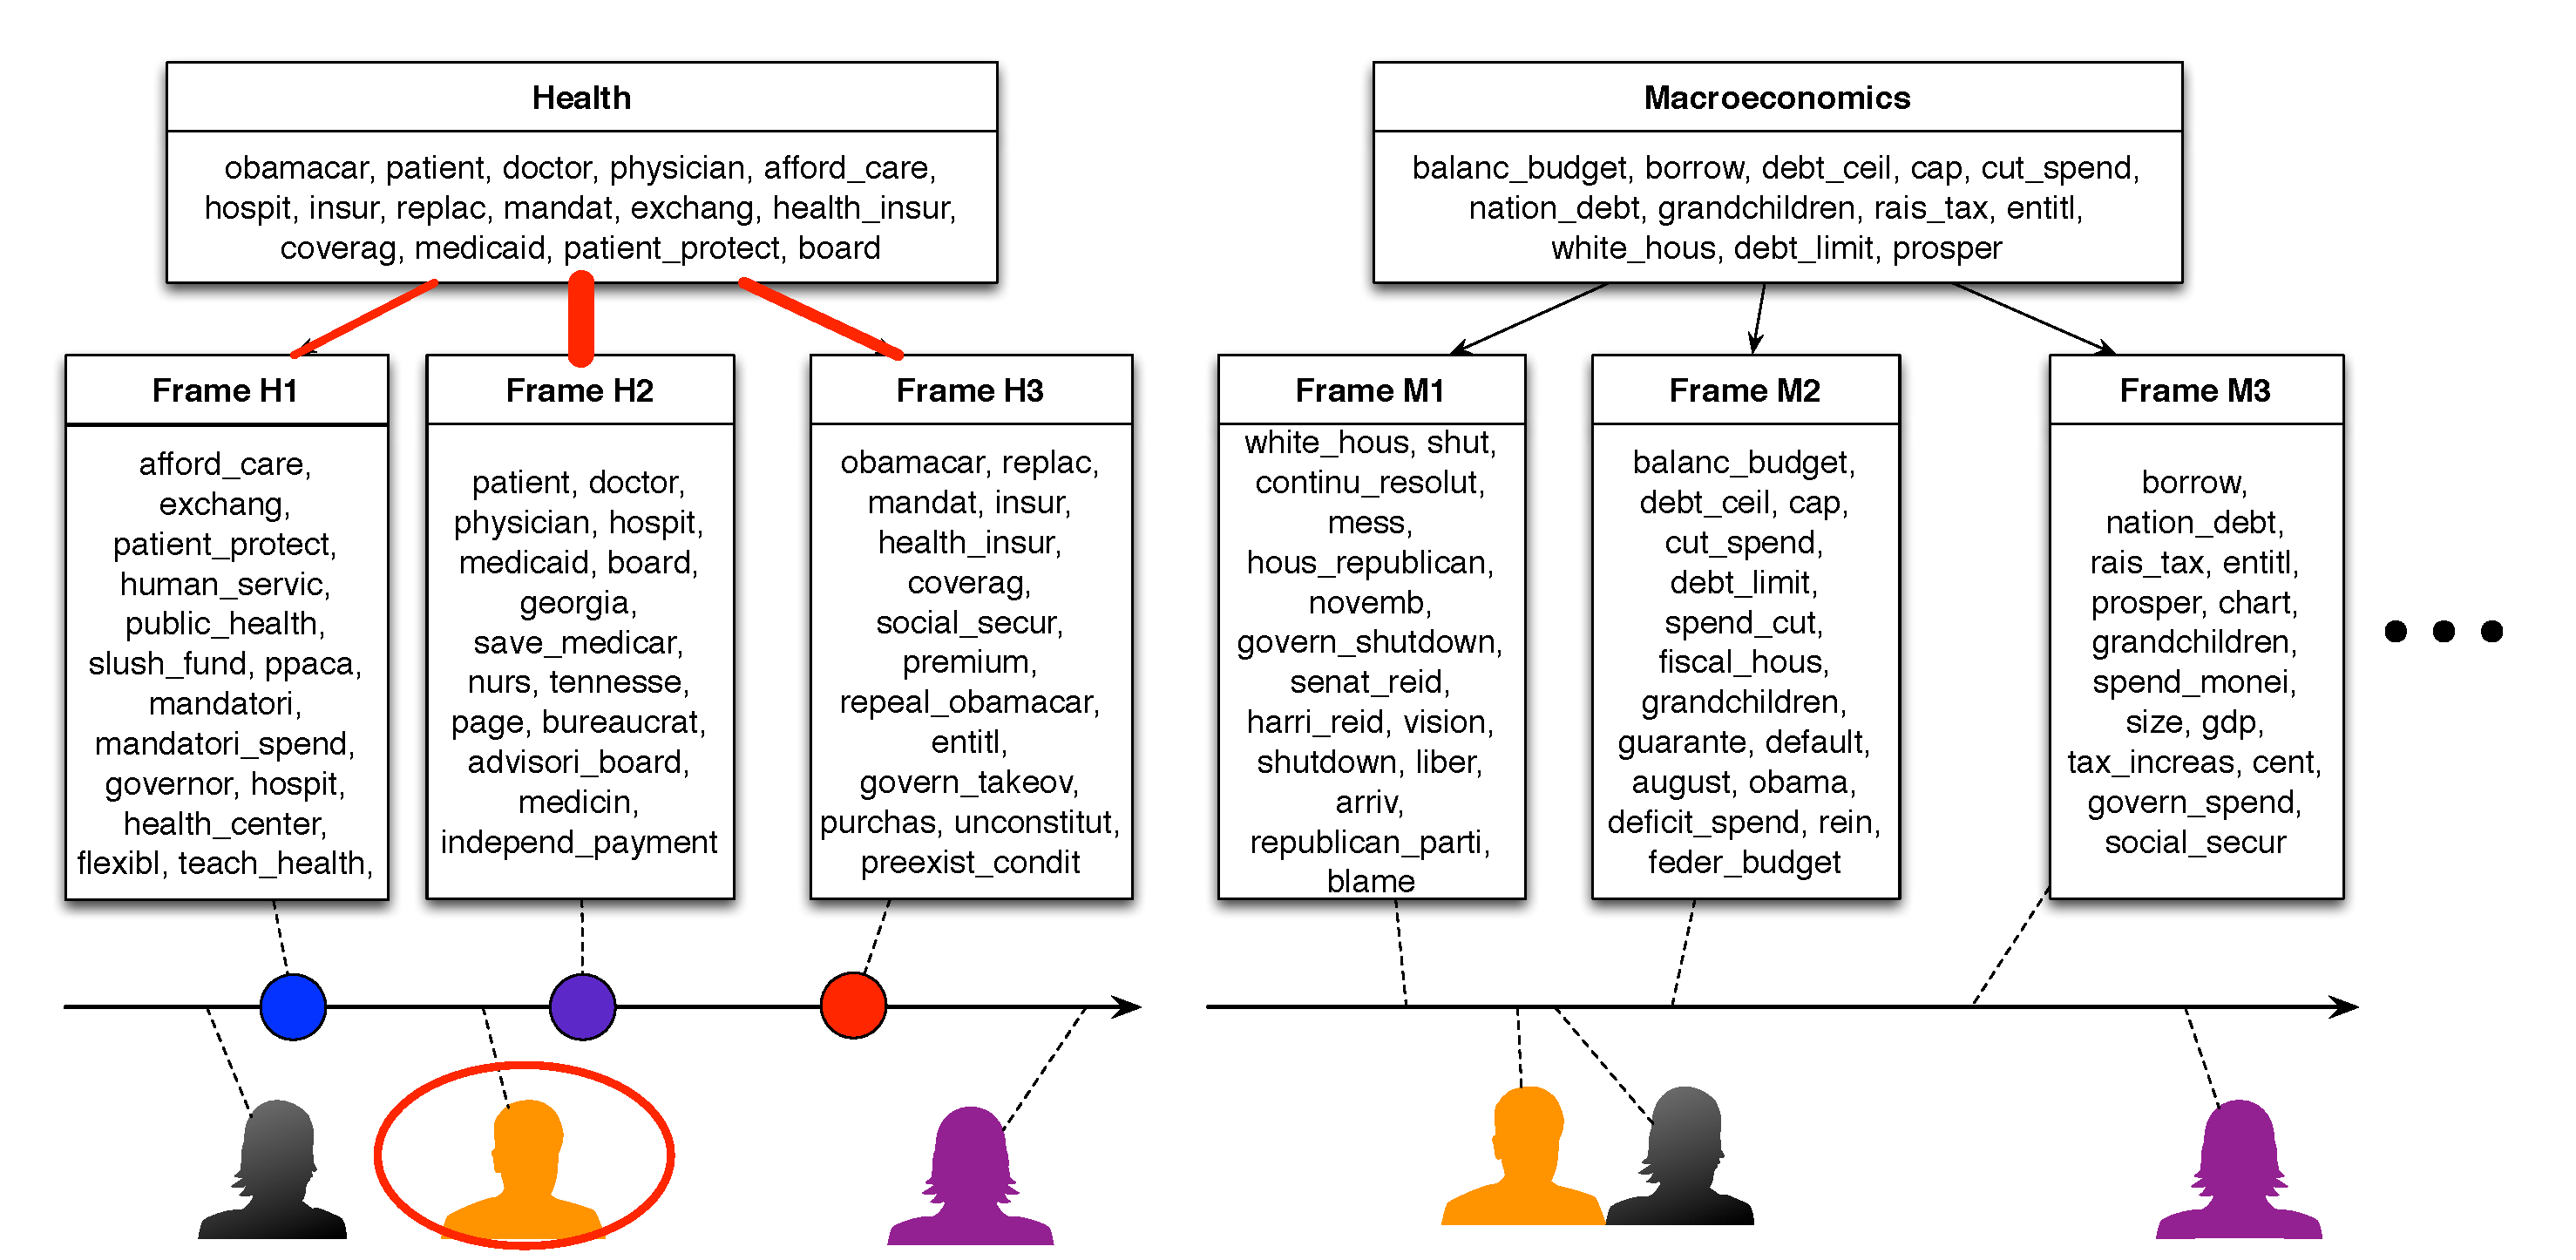
\includegraphics[width=.8\textwidth]{teaparty/figures/s5/modeling_idealpoint}
    \end{center}
    }
}

\frame{
\frametitle{Evaluation: Tea Party in the House}
    \begin{block}{The Tea Party}
    \small
    \begin{itemize*}
      \item Recent American political movement supporting more freedom, smaller government, lower tax
      \item Played an important role in recent electoral politics, especially within the Republican
      Party
    \end{itemize*}
    \end{block}

    \pause
    \vspace{-.2cm}
    \begin{block}{Data}
    \small
    \begin{itemize*}
      \item 240 Republican Representatives in the 112\textsuperscript{th} U.S. House
      \item 60 are members of the Tea Party Caucus (self-identified)
      \item 60 key votes selected by Freedom Works (2011-2012)
      \item Speeches, bill text and voting records from the Library of Congress
    \end{itemize*}
    \end{block}
}

\section{How They Vote}

\frame{
    \frametitle{One-dimensional Ideal Points}
    \begin{columns}
      \column{.49\textwidth}
      \vspace{-.5cm}
      \begin{center}
        \includegraphics<1>[width=.8\textwidth]{teaparty/figures/s5/bottom_0}%
        \includegraphics<2-3>[width=.8\textwidth]{teaparty/figures/s5/bottom_1}%
      \end{center}
        \only<4>{
        \vspace{-1cm}
            \begin{block}{}
            \small
            \begin{itemize}
              \item \textbf{Flake} and \textbf{Amash} didn't self-identify as members of the
                  Tea Party Caucus but have been endorsed by other Tea Party organizations
            \end{itemize}
            \end{block}

            \vspace{-.2cm}

            \begin{block}{}
            \begin{center}
              \includegraphics<4>[width=.65\textwidth]{teaparty/figures/s5/new_republic.png}%
            \end{center}
            \vspace{-.5cm}
            \footnotesize
                ``Some 46 House members and six senators had been [Tea Party] \dots In addition, there were about 18 other House members like Trey Gowdy, Mark
Meadows, and \redtext{Justin Amash}, and several senators, including \redtext{Jeff Flake} and Pat
Toomey, \redtext{who owed their election to support from the Tea Party and its Washington
allies}.''
            \end{block}
        }
      \column{.49\textwidth}
      \vspace{-.5cm}
      \begin{center}
        \includegraphics<1>[width=.8\textwidth]{teaparty/figures/s5/top_0}%
        \includegraphics<2,4>[width=.8\textwidth]{teaparty/figures/s5/top_1}%
      \end{center}
        \only<3>{
        \vspace{-1cm}
            \begin{block}{}
            \small
                \begin{itemize}
                  \item \textbf{Alexander} and \textbf{Crenshaw}'s votes only agree with
                      Freedom Works 48\% and 50\% respectively
                  \item Both voted for raising the debt ceiling and are listed as ``\alert<3>{traitor}''
                \end{itemize}
            \end{block}
            \includegraphics<3>[width=\textwidth]{teaparty/figures/s5/traitor.png}
        }
    \end{columns}
}

\frame{
    \frametitle{Multi-dimensional Ideal Points}
    \begin{figure}
      \centering
        %\includegraphics<1>[width=.7\textwidth]{teaparty/figures/s5/multdim_ip_112}%
        \includegraphics<1->[width=\textwidth]{teaparty/figures/s5/mult_ip_top}%
    \end{figure}
    \only<2->{
        \begin{block}{}
            Freedom Works' key votes on most highly polarized dimensions are about government spending
        \end{block}
    }
}

\section{Predicting Membership}

\frame{
    \frametitle{Tea Party Caucus Membership Prediction}
    \begin{block}{Experiment setup}
    \begin{itemize}
    \small
      \item Task: Binary classification of whether a legislator is a member of the Tea Party Caucus
      \item Evaluation metric: AUC-ROC
      \item Classifier: SVM$^{light}$
      \item Five-fold stratified cross-validation
    \end{itemize}
    \end{block}

    \pause

    \begin{block}{Features}
    \begin{itemize}
    \small
      \item Text-based features: normalized term frequency (\textbf{TF}) and \textbf{TF-IDF}
      \item \textbf{Vote}: binary features
      \item \textbf{HIPTM}: features extracted from our model including
      \begin{itemize}
        \item $K$-dim ideal point $u \subtwo ak$ estimated from both votes and text
        \item $K$-dim ideal point estimated from text only $\bm \eta_k^T \hat{\bm \psi} \subtwo ak$
        \item $B$ probabilities estimating $a$'s votes $\Phi(x_b \sum_{k=1}^K \vartheta \subtwo bk u \subtwo ak +
          y_b)$
      \end{itemize}
    \end{itemize}
    \end{block}
}

\frame{
    \frametitle{Tea Party Caucus Membership Prediction: Votes \& Text}
    \begin{center}
        \includegraphics<1>[width=\textwidth]{teaparty/figures/s5/votetext_1}
        \includegraphics<2>[width=\textwidth]{teaparty/figures/s5/votetext_2}
        \includegraphics<3>[width=\textwidth]{teaparty/figures/s5/votetext_3}
        \includegraphics<4>[width=\textwidth]{teaparty/figures/s5/votetext_4}
        \includegraphics<5>[width=\textwidth]{teaparty/figures/s5/votetext_5}
        \includegraphics<6>[width=\textwidth]{teaparty/figures/s5/votetext_6}
    \end{center}
}

\frame{
    \frametitle{Tea Party Caucus Membership Prediction: Text Only}
      \begin{center}
        \includegraphics<1>[width=\textwidth]{teaparty/figures/s5/textonly_1}
        \includegraphics<2->[width=\textwidth]{teaparty/figures/s5/textonly_2}
      \end{center}

%      \begin{block}{}
%        Vote-based features are not needed at test time, so this model makes it possible to do better
%prediction even for people who have no voting record in Congress
%        \begin{itemize}
%          \item e.g., new members of Congress or political candidates.
%        \end{itemize}
%      \end{block}
}

\section{How They Talk}

\begin{frame}{Framing Healthcare}
	\gfx{health}{.8}
\end{frame}

\begin{frame}{Framing Macroeconomics}
	\gfx{macroeconomics}{.8}
\end{frame}


\begin{frame}{Polarization}
	\gfx{polarization}{.8}
\end{frame}

\section{Conclusion}




\end{document}
